\documentclass[twoside]{book}

% Packages required by doxygen
\usepackage{fixltx2e}
\usepackage{calc}
\usepackage{doxygen}
\usepackage[export]{adjustbox} % also loads graphicx
\usepackage{graphicx}
\usepackage[utf8]{inputenc}
\usepackage{makeidx}
\usepackage{multicol}
\usepackage{multirow}
\PassOptionsToPackage{warn}{textcomp}
\usepackage{textcomp}
\usepackage[nointegrals]{wasysym}
\usepackage[table]{xcolor}

% Font selection
\usepackage[T1]{fontenc}
\usepackage[scaled=.90]{helvet}
\usepackage{courier}
\usepackage{amssymb}
\usepackage{sectsty}
\renewcommand{\familydefault}{\sfdefault}
\allsectionsfont{%
  \fontseries{bc}\selectfont%
  \color{darkgray}%
}
\renewcommand{\DoxyLabelFont}{%
  \fontseries{bc}\selectfont%
  \color{darkgray}%
}
\newcommand{\+}{\discretionary{\mbox{\scriptsize$\hookleftarrow$}}{}{}}

% Page & text layout
\usepackage{geometry}
\geometry{%
  a4paper,%
  top=2.5cm,%
  bottom=2.5cm,%
  left=2.5cm,%
  right=2.5cm%
}
\tolerance=750
\hfuzz=15pt
\hbadness=750
\setlength{\emergencystretch}{15pt}
\setlength{\parindent}{0cm}
\setlength{\parskip}{3ex plus 2ex minus 2ex}
\makeatletter
\renewcommand{\paragraph}{%
  \@startsection{paragraph}{4}{0ex}{-1.0ex}{1.0ex}{%
    \normalfont\normalsize\bfseries\SS@parafont%
  }%
}
\renewcommand{\subparagraph}{%
  \@startsection{subparagraph}{5}{0ex}{-1.0ex}{1.0ex}{%
    \normalfont\normalsize\bfseries\SS@subparafont%
  }%
}
\makeatother

% Headers & footers
\usepackage{fancyhdr}
\pagestyle{fancyplain}
\fancyhead[LE]{\fancyplain{}{\bfseries\thepage}}
\fancyhead[CE]{\fancyplain{}{}}
\fancyhead[RE]{\fancyplain{}{\bfseries\leftmark}}
\fancyhead[LO]{\fancyplain{}{\bfseries\rightmark}}
\fancyhead[CO]{\fancyplain{}{}}
\fancyhead[RO]{\fancyplain{}{\bfseries\thepage}}
\fancyfoot[LE]{\fancyplain{}{}}
\fancyfoot[CE]{\fancyplain{}{}}
\fancyfoot[RE]{\fancyplain{}{\bfseries\scriptsize Generated by Doxygen }}
\fancyfoot[LO]{\fancyplain{}{\bfseries\scriptsize Generated by Doxygen }}
\fancyfoot[CO]{\fancyplain{}{}}
\fancyfoot[RO]{\fancyplain{}{}}
\renewcommand{\footrulewidth}{0.4pt}
\renewcommand{\chaptermark}[1]{%
  \markboth{#1}{}%
}
\renewcommand{\sectionmark}[1]{%
  \markright{\thesection\ #1}%
}

% Indices & bibliography
\usepackage{natbib}
\usepackage[titles]{tocloft}
\setcounter{tocdepth}{3}
\setcounter{secnumdepth}{5}
\makeindex

% Hyperlinks (required, but should be loaded last)
\usepackage{ifpdf}
\ifpdf
  \usepackage[pdftex,pagebackref=true]{hyperref}
\else
  \usepackage[ps2pdf,pagebackref=true]{hyperref}
\fi
\hypersetup{%
  colorlinks=true,%
  linkcolor=blue,%
  citecolor=blue,%
  unicode%
}

% Custom commands
\newcommand{\clearemptydoublepage}{%
  \newpage{\pagestyle{empty}\cleardoublepage}%
}

\usepackage{caption}
\captionsetup{labelsep=space,justification=centering,font={bf},singlelinecheck=off,skip=4pt,position=top}

%===== C O N T E N T S =====

\begin{document}

% Titlepage & ToC
\hypersetup{pageanchor=false,
             bookmarksnumbered=true,
             pdfencoding=unicode
            }
\pagenumbering{alph}
\begin{titlepage}
\vspace*{7cm}
\begin{center}%
{\Large Telescope Control System }\\
\vspace*{1cm}
{\large Generated by Doxygen 1.8.14}\\
\end{center}
\end{titlepage}
\clearemptydoublepage
\pagenumbering{roman}
\tableofcontents
\clearemptydoublepage
\pagenumbering{arabic}
\hypersetup{pageanchor=true}

%--- Begin generated contents ---
\chapter{Telescope Control System}
\label{md_readme}
\Hypertarget{md_readme}
Telescope Control System is a C++ program for the Raspberry Pi. The program communicates with a connected Arduino that reorients a telescope. The telescope can be reoriented using the inputted horizontal celestial coordinates from the Qt Interface on the Pi.

\subsection*{Getting Started}

The instructions below will allow you to compile the project and run it on the Raspberry Pi.

\subsubsection*{Prerequisites}

Install the Qt libraries using {\ttfamily apt}\+: 
\begin{DoxyCode}
sudo apt install qt5-default
\end{DoxyCode}


\subsubsection*{Installation}

Generate the {\ttfamily Makefile} using the existing project {\ttfamily telescope.\+pro}\+: 
\begin{DoxyCode}
qmake telescope.pro
\end{DoxyCode}


Build the program\+: 
\begin{DoxyCode}
make
\end{DoxyCode}


\subsection*{Usage}

After installation just run the program from the directory {\ttfamily group25}\+: 
\begin{DoxyCode}
./telescope
\end{DoxyCode}


\subsection*{Development}

If you wish to build the program with the files you are developing, edit the {\ttfamily telescope.\+pro} file to include {\ttfamily .h} and {\ttfamily .cpp} files. The {\ttfamily telescope.\+pro} file should look like this\+: 
\begin{DoxyCode}
QT += widgets

TEMPLATE = app
TARGET = telescope
INCLUDEPATH += .

DEFINES += QT\_DEPRECATED\_WARNINGS


# Input
HEADERS += backendwrapper.h \(\backslash\)
           telescopeui.h
FORMS += raspberrypiutility.ui
SOURCES += backendwrapper.cpp \(\backslash\)
           main.cpp \(\backslash\)
           telescopeui.cpp
RESOURCES += raspberrypiutility.qrc
\end{DoxyCode}


Qt {\ttfamily .ui} files should be appended to {\ttfamily F\+O\+R\+MS}, C++ header {\ttfamily .h} files to {\ttfamily H\+E\+A\+D\+E\+RS}, C++ files {\ttfamily .cpp} to {\ttfamily S\+O\+U\+R\+C\+ES}.

To generate a fresh Qt project file\+: 
\begin{DoxyCode}
qmake -project -o telescope.pro
\end{DoxyCode}
 Edit {\ttfamily telescope.\+pro} to include\+: 
\begin{DoxyCode}
QT += widgets
\end{DoxyCode}
 
\chapter{Hierarchical Index}
\section{Class Hierarchy}
This inheritance list is sorted roughly, but not completely, alphabetically\+:\begin{DoxyCompactList}
\item \contentsline{section}{Angle}{\pageref{classAngle}}{}
\item \contentsline{section}{Backend}{\pageref{classBackend}}{}
\item \contentsline{section}{Bridge\+In$<$ Args $>$}{\pageref{classBridgeIn}}{}
\item \contentsline{section}{Bridge\+In$<$ double, double $>$}{\pageref{classBridgeIn}}{}
\begin{DoxyCompactList}
\item \contentsline{section}{Control\+In}{\pageref{classControlIn}}{}
\end{DoxyCompactList}
\item \contentsline{section}{Bridge\+In$<$ std\+:\+:string $>$}{\pageref{classBridgeIn}}{}
\begin{DoxyCompactList}
\item \contentsline{section}{Celestial\+In}{\pageref{classCelestialIn}}{}
\end{DoxyCompactList}
\item \contentsline{section}{Bridge\+Out$<$ Args $>$}{\pageref{classBridgeOut}}{}
\item \contentsline{section}{Bridge\+Out$<$ double, double $>$}{\pageref{classBridgeOut}}{}
\begin{DoxyCompactList}
\item \contentsline{section}{Control\+Out}{\pageref{classControlOut}}{}
\end{DoxyCompactList}
\item \contentsline{section}{Bridge\+Out$<$ rightasc, declination $>$}{\pageref{classBridgeOut}}{}
\begin{DoxyCompactList}
\item \contentsline{section}{Celestial\+Out}{\pageref{classCelestialOut}}{}
\end{DoxyCompactList}
\item \contentsline{section}{ce}{\pageref{classce}}{}
\item \contentsline{section}{Celestial\+DB}{\pageref{structCelestialDB}}{}
\item \contentsline{section}{declination}{\pageref{structdeclination}}{}
\item \contentsline{section}{Equatorial\+Coordinates}{\pageref{classEquatorialCoordinates}}{}
\item \contentsline{section}{Fake\+Serial}{\pageref{structFakeSerial}}{}
\item \contentsline{section}{Full\+Step\+Controller}{\pageref{classFullStepController}}{}
\item \contentsline{section}{Horizontal\+Coordinates}{\pageref{classHorizontalCoordinates}}{}
\item \contentsline{section}{Manual\+Translation}{\pageref{classManualTranslation}}{}
\item \contentsline{section}{Motor\+Control}{\pageref{structMotorControl}}{}
\item \contentsline{section}{Pin}{\pageref{classPin}}{}
\item \contentsline{section}{Planet}{\pageref{classPlanet}}{}
\item Q\+Main\+Window\begin{DoxyCompactList}
\item \contentsline{section}{Telescope\+UI}{\pageref{classTelescopeUI}}{}
\end{DoxyCompactList}
\item \contentsline{section}{Raspberry\+Pi\+Utility}{\pageref{classRaspberryPiUtility}}{}
\item \contentsline{section}{rightasc}{\pageref{structrightasc}}{}
\item \contentsline{section}{Serial\+Port}{\pageref{classSerialPort}}{}
\item \contentsline{section}{Star}{\pageref{classStar}}{}
\item \contentsline{section}{Stepper}{\pageref{classStepper}}{}
\item \contentsline{section}{tmc}{\pageref{classtmc}}{}
\item \contentsline{section}{web}{\pageref{classweb}}{}
\end{DoxyCompactList}

\chapter{Class Index}
\section{Class List}
Here are the classes, structs, unions and interfaces with brief descriptions\+:\begin{DoxyCompactList}
\item\contentsline{section}{\mbox{\hyperlink{classAngle}{Angle}} }{\pageref{classAngle}}{}
\item\contentsline{section}{\mbox{\hyperlink{classBackend}{Backend}} \\*Primary class for wrapping together all the backend objects and functions used to talk between those objects }{\pageref{classBackend}}{}
\item\contentsline{section}{\mbox{\hyperlink{classBridgeIn}{Bridge\+In$<$ Args $>$}} }{\pageref{classBridgeIn}}{}
\item\contentsline{section}{\mbox{\hyperlink{classBridgeOut}{Bridge\+Out$<$ Args $>$}} }{\pageref{classBridgeOut}}{}
\item\contentsline{section}{\mbox{\hyperlink{classce}{ce}} }{\pageref{classce}}{}
\item\contentsline{section}{\mbox{\hyperlink{structCelestialDB}{Celestial\+DB}} }{\pageref{structCelestialDB}}{}
\item\contentsline{section}{\mbox{\hyperlink{classCelestialIn}{Celestial\+In}} }{\pageref{classCelestialIn}}{}
\item\contentsline{section}{\mbox{\hyperlink{classCelestialOut}{Celestial\+Out}} }{\pageref{classCelestialOut}}{}
\item\contentsline{section}{\mbox{\hyperlink{classControlIn}{Control\+In}} }{\pageref{classControlIn}}{}
\item\contentsline{section}{\mbox{\hyperlink{classControlOut}{Control\+Out}} }{\pageref{classControlOut}}{}
\item\contentsline{section}{\mbox{\hyperlink{structdeclination}{declination}} }{\pageref{structdeclination}}{}
\item\contentsline{section}{\mbox{\hyperlink{classEquatorialCoordinates}{Equatorial\+Coordinates}} }{\pageref{classEquatorialCoordinates}}{}
\item\contentsline{section}{\mbox{\hyperlink{structFakeSerial}{Fake\+Serial}} }{\pageref{structFakeSerial}}{}
\item\contentsline{section}{\mbox{\hyperlink{classFullStepController}{Full\+Step\+Controller}} }{\pageref{classFullStepController}}{}
\item\contentsline{section}{\mbox{\hyperlink{classHorizontalCoordinates}{Horizontal\+Coordinates}} }{\pageref{classHorizontalCoordinates}}{}
\item\contentsline{section}{\mbox{\hyperlink{classManualTranslation}{Manual\+Translation}} }{\pageref{classManualTranslation}}{}
\item\contentsline{section}{\mbox{\hyperlink{structMotorControl}{Motor\+Control}} }{\pageref{structMotorControl}}{}
\item\contentsline{section}{\mbox{\hyperlink{classPin}{Pin}} }{\pageref{classPin}}{}
\item\contentsline{section}{\mbox{\hyperlink{classPlanet}{Planet}} }{\pageref{classPlanet}}{}
\item\contentsline{section}{\mbox{\hyperlink{classRaspberryPiUtility}{Raspberry\+Pi\+Utility}} }{\pageref{classRaspberryPiUtility}}{}
\item\contentsline{section}{\mbox{\hyperlink{structrightasc}{rightasc}} }{\pageref{structrightasc}}{}
\item\contentsline{section}{\mbox{\hyperlink{classSerialPort}{Serial\+Port}} }{\pageref{classSerialPort}}{}
\item\contentsline{section}{\mbox{\hyperlink{classStar}{Star}} }{\pageref{classStar}}{}
\item\contentsline{section}{\mbox{\hyperlink{classStepper}{Stepper}} }{\pageref{classStepper}}{}
\item\contentsline{section}{\mbox{\hyperlink{classTelescopeUI}{Telescope\+UI}} \\*$<$ Qt template UI generated using Qt Creator }{\pageref{classTelescopeUI}}{}
\item\contentsline{section}{\mbox{\hyperlink{classtmc}{tmc}} }{\pageref{classtmc}}{}
\item\contentsline{section}{\mbox{\hyperlink{classweb}{web}} }{\pageref{classweb}}{}
\end{DoxyCompactList}

\chapter{File Index}
\section{File List}
Here is a list of all documented files with brief descriptions\+:\begin{DoxyCompactList}
\item\contentsline{section}{\mbox{\hyperlink{Angle_8cpp}{Angle.\+cpp}} \\*\mbox{\hyperlink{classAngle}{Angle}} class represents angular measurements and allows conversion between different units }{\pageref{Angle_8cpp}}{}
\item\contentsline{section}{\mbox{\hyperlink{Angle_8h}{Angle.\+h}} \\*\mbox{\hyperlink{classAngle}{Angle}} class represents angular measurements and allows conversion between different units }{\pageref{Angle_8h}}{}
\item\contentsline{section}{{\bfseries backendwrapper.\+h} }{\pageref{backendwrapper_8h}}{}
\item\contentsline{section}{{\bfseries bridgein.\+h} }{\pageref{bridgein_8h}}{}
\item\contentsline{section}{{\bfseries bridgeout.\+h} }{\pageref{bridgeout_8h}}{}
\item\contentsline{section}{\mbox{\hyperlink{celestialdb_8h}{celestialdb.\+h}} \\*Implements Celestial Database }{\pageref{celestialdb_8h}}{}
\item\contentsline{section}{\mbox{\hyperlink{celestialin_8h}{celestialin.\+h}} \\*Bridge between celestialdb class and UI }{\pageref{celestialin_8h}}{}
\item\contentsline{section}{{\bfseries celestialout.\+h} }{\pageref{celestialout_8h}}{}
\item\contentsline{section}{\mbox{\hyperlink{control_8h}{control.\+h}} \\*A\+PI for the Telescope Motor Control there is no function to read the current coordinates as the design does not allow the motor control to be polled }{\pageref{control_8h}}{}
\item\contentsline{section}{{\bfseries controlin.\+h} }{\pageref{controlin_8h}}{}
\item\contentsline{section}{{\bfseries controlout.\+h} }{\pageref{controlout_8h}}{}
\item\contentsline{section}{\mbox{\hyperlink{coordencoder_8h}{coordencoder.\+h}} \\*Methods for converting coordinates into integers and bytes }{\pageref{coordencoder_8h}}{}
\item\contentsline{section}{\mbox{\hyperlink{coordinates_8h}{coordinates.\+h}} \\*Structures for equatorial coordinates }{\pageref{coordinates_8h}}{}
\item\contentsline{section}{\mbox{\hyperlink{downloadpage_8h}{downloadpage.\+h}} \\*Implements retrieval of webpage data }{\pageref{downloadpage_8h}}{}
\item\contentsline{section}{\mbox{\hyperlink{EquatorialCoordinates_8h}{Equatorial\+Coordinates.\+h}} \\*\mbox{\hyperlink{classEquatorialCoordinates}{Equatorial\+Coordinates}} class represents celestial coordinates in the equatorial (right ascension-\/declination) system }{\pageref{EquatorialCoordinates_8h}}{}
\item\contentsline{section}{\mbox{\hyperlink{fakeserial_8h}{fakeserial.\+h}} \\*\mbox{\hyperlink{structFakeSerial}{Fake\+Serial}} class imitates some output from the serial port to use for testing purposes it effectively replaces the serial driver }{\pageref{fakeserial_8h}}{}
\item\contentsline{section}{\mbox{\hyperlink{FullStepController_8h}{Full\+Step\+Controller.\+h}} \\*Implements stepper motor controller }{\pageref{FullStepController_8h}}{}
\item\contentsline{section}{\mbox{\hyperlink{gpio_8h}{gpio.\+h}} \\*Each object instantiated from this class will control a G\+P\+IO pin }{\pageref{gpio_8h}}{}
\item\contentsline{section}{\mbox{\hyperlink{HorizontalCoordinates_8cpp}{Horizontal\+Coordinates.\+cpp}} \\*\mbox{\hyperlink{classHorizontalCoordinates}{Horizontal\+Coordinates}} class represents celestial coordinates in the horizontal (altitude-\/azimuth) system }{\pageref{HorizontalCoordinates_8cpp}}{}
\item\contentsline{section}{\mbox{\hyperlink{HorizontalCoordinates_8h}{Horizontal\+Coordinates.\+h}} \\*\mbox{\hyperlink{classHorizontalCoordinates}{Horizontal\+Coordinates}} class represents celestial coordinates in the horizontal (altitude-\/azimuth) system }{\pageref{HorizontalCoordinates_8h}}{}
\item\contentsline{section}{\mbox{\hyperlink{main_8cpp}{main.\+cpp}} \\*Main program for Telescope\+Control\+System }{\pageref{main_8cpp}}{}
\item\contentsline{section}{\mbox{\hyperlink{motorcontrol_8h}{motorcontrol.\+h}} \\*\mbox{\hyperlink{structMotorControl}{Motor\+Control}} class acts as the driver interface; it ensures incoming and outgoing data is normalized and within range before it is injested by the driver }{\pageref{motorcontrol_8h}}{}
\item\contentsline{section}{\mbox{\hyperlink{planet_8h}{planet.\+h}} \\*Part of Celestial database. Retrieves planet object from webpage }{\pageref{planet_8h}}{}
\item\contentsline{section}{\mbox{\hyperlink{serialport_8h}{serialport.\+h}} \\*Driver for the Serial port enabling reading and writing, this is done in a blocking way }{\pageref{serialport_8h}}{}
\item\contentsline{section}{\mbox{\hyperlink{star_8h}{star.\+h}} \\*Part of Celestial Database. Retrives star object from webpage }{\pageref{star_8h}}{}
\item\contentsline{section}{\mbox{\hyperlink{Stepper_8h}{Stepper.\+h}} \\*Part of motor control. Manages stepper motor }{\pageref{Stepper_8h}}{}
\item\contentsline{section}{{\bfseries telescopeui.\+h} }{\pageref{telescopeui_8h}}{}
\item\contentsline{section}{{\bfseries translation.\+h} }{\pageref{translation_8h}}{}
\end{DoxyCompactList}

\chapter{Class Documentation}
\hypertarget{classAngle}{}\section{Angle Class Reference}
\label{classAngle}\index{Angle@{Angle}}
\subsection*{Public Member Functions}
\begin{DoxyCompactItemize}
\item 
\mbox{\Hypertarget{classAngle_aca3c6e1519b40835d31736430ca082a9}\label{classAngle_aca3c6e1519b40835d31736430ca082a9}} 
\mbox{\hyperlink{classAngle_aca3c6e1519b40835d31736430ca082a9}{Angle}} ()
\begin{DoxyCompactList}\small\item\em null constructor method for an \mbox{\hyperlink{classAngle}{Angle}} -- does not create a meaningful \mbox{\hyperlink{classAngle}{Angle}} \end{DoxyCompactList}\item 
\mbox{\hyperlink{classAngle_a0c77cde78d872c2353b7b583e5928230}{Angle}} (double radians)
\begin{DoxyCompactList}\small\item\em constructor method for an \mbox{\hyperlink{classAngle}{Angle}} using radians \end{DoxyCompactList}\item 
\mbox{\hyperlink{classAngle_aaddbbb2df503cad123ceec60df3778d7}{Angle}} (double degrees, double arcminutes, double arcseconds)
\begin{DoxyCompactList}\small\item\em constructor method for an \mbox{\hyperlink{classAngle}{Angle}} using degrees, arcminutes, arcseconds \end{DoxyCompactList}\item 
double \mbox{\hyperlink{classAngle_af8f8715184904ea14d1e951be1f8d60c}{get\+\_\+radians}} ()
\begin{DoxyCompactList}\small\item\em getter method for the \mbox{\hyperlink{classAngle}{Angle}}, measured in radians \end{DoxyCompactList}\item 
double \mbox{\hyperlink{classAngle_a592d871a119dd6470e3af13e76debb07}{get\+\_\+degrees}} ()
\begin{DoxyCompactList}\small\item\em getter method for the \mbox{\hyperlink{classAngle}{Angle}}, measured in degrees \end{DoxyCompactList}\item 
double \mbox{\hyperlink{classAngle_a2664851f26ad091294ed0dd2737026b2}{get\+\_\+arcminutes}} ()
\begin{DoxyCompactList}\small\item\em getter method for the \mbox{\hyperlink{classAngle}{Angle}}, measured in arcminutes \end{DoxyCompactList}\item 
double \mbox{\hyperlink{classAngle_a64ecc29aea0d9487058a6bec3f141e54}{get\+\_\+arcseconds}} ()
\begin{DoxyCompactList}\small\item\em getter method for the \mbox{\hyperlink{classAngle}{Angle}}, measured in arcseconds \end{DoxyCompactList}\item 
std\+::map$<$ std\+::string, double $>$ \mbox{\hyperlink{classAngle_a5425dc27480fec42fb3046378a70920e}{get\+\_\+degrees\+\_\+arcminutes\+\_\+arcseconds}} ()
\begin{DoxyCompactList}\small\item\em getter method for the \mbox{\hyperlink{classAngle}{Angle}}, measured in (degrees, arcminutes, arcseconds) -- (e.\+g. 10 deg 37 arcmin 12.\+32 arcsec) \end{DoxyCompactList}\end{DoxyCompactItemize}
\subsection*{Private Attributes}
\begin{DoxyCompactItemize}
\item 
\mbox{\Hypertarget{classAngle_a0985c4f08e7c075f29db63e5e313fe1f}\label{classAngle_a0985c4f08e7c075f29db63e5e313fe1f}} 
double \mbox{\hyperlink{classAngle_a0985c4f08e7c075f29db63e5e313fe1f}{\+\_\+angle\+\_\+radians}}
\begin{DoxyCompactList}\small\item\em internal representation of the angle \end{DoxyCompactList}\end{DoxyCompactItemize}


\subsection{Constructor \& Destructor Documentation}
\mbox{\Hypertarget{classAngle_a0c77cde78d872c2353b7b583e5928230}\label{classAngle_a0c77cde78d872c2353b7b583e5928230}} 
\index{Angle@{Angle}!Angle@{Angle}}
\index{Angle@{Angle}!Angle@{Angle}}
\subsubsection{\texorpdfstring{Angle()}{Angle()}\hspace{0.1cm}{\footnotesize\ttfamily [1/2]}}
{\footnotesize\ttfamily Angle\+::\+Angle (\begin{DoxyParamCaption}\item[{double}]{radians }\end{DoxyParamCaption})}



constructor method for an \mbox{\hyperlink{classAngle}{Angle}} using radians 


\begin{DoxyParams}{Parameters}
{\em radians} & represents the angle in radians \\
\hline
\end{DoxyParams}
\mbox{\Hypertarget{classAngle_aaddbbb2df503cad123ceec60df3778d7}\label{classAngle_aaddbbb2df503cad123ceec60df3778d7}} 
\index{Angle@{Angle}!Angle@{Angle}}
\index{Angle@{Angle}!Angle@{Angle}}
\subsubsection{\texorpdfstring{Angle()}{Angle()}\hspace{0.1cm}{\footnotesize\ttfamily [2/2]}}
{\footnotesize\ttfamily Angle\+::\+Angle (\begin{DoxyParamCaption}\item[{double}]{degrees,  }\item[{double}]{arcminutes,  }\item[{double}]{arcseconds }\end{DoxyParamCaption})}



constructor method for an \mbox{\hyperlink{classAngle}{Angle}} using degrees, arcminutes, arcseconds 


\begin{DoxyParams}{Parameters}
{\em degrees} & represents the degree part of the \mbox{\hyperlink{classAngle}{Angle}} \\
\hline
{\em arcminutes} & represents the arcminutes part of the \mbox{\hyperlink{classAngle}{Angle}} \\
\hline
{\em arcseconds} & represents the arcseconds part of \mbox{\hyperlink{classAngle}{Angle}} \\
\hline
\end{DoxyParams}


\subsection{Member Function Documentation}
\mbox{\Hypertarget{classAngle_a2664851f26ad091294ed0dd2737026b2}\label{classAngle_a2664851f26ad091294ed0dd2737026b2}} 
\index{Angle@{Angle}!get\+\_\+arcminutes@{get\+\_\+arcminutes}}
\index{get\+\_\+arcminutes@{get\+\_\+arcminutes}!Angle@{Angle}}
\subsubsection{\texorpdfstring{get\+\_\+arcminutes()}{get\_arcminutes()}}
{\footnotesize\ttfamily double Angle\+::get\+\_\+arcminutes (\begin{DoxyParamCaption}{ }\end{DoxyParamCaption})}



getter method for the \mbox{\hyperlink{classAngle}{Angle}}, measured in arcminutes 

\begin{DoxyReturn}{Returns}
the \mbox{\hyperlink{classAngle}{Angle}}, measured in arcminutes 
\end{DoxyReturn}
\mbox{\Hypertarget{classAngle_a64ecc29aea0d9487058a6bec3f141e54}\label{classAngle_a64ecc29aea0d9487058a6bec3f141e54}} 
\index{Angle@{Angle}!get\+\_\+arcseconds@{get\+\_\+arcseconds}}
\index{get\+\_\+arcseconds@{get\+\_\+arcseconds}!Angle@{Angle}}
\subsubsection{\texorpdfstring{get\+\_\+arcseconds()}{get\_arcseconds()}}
{\footnotesize\ttfamily double Angle\+::get\+\_\+arcseconds (\begin{DoxyParamCaption}{ }\end{DoxyParamCaption})}



getter method for the \mbox{\hyperlink{classAngle}{Angle}}, measured in arcseconds 

\begin{DoxyReturn}{Returns}
the \mbox{\hyperlink{classAngle}{Angle}}, measured in arcseconds 
\end{DoxyReturn}
\mbox{\Hypertarget{classAngle_a592d871a119dd6470e3af13e76debb07}\label{classAngle_a592d871a119dd6470e3af13e76debb07}} 
\index{Angle@{Angle}!get\+\_\+degrees@{get\+\_\+degrees}}
\index{get\+\_\+degrees@{get\+\_\+degrees}!Angle@{Angle}}
\subsubsection{\texorpdfstring{get\+\_\+degrees()}{get\_degrees()}}
{\footnotesize\ttfamily double Angle\+::get\+\_\+degrees (\begin{DoxyParamCaption}{ }\end{DoxyParamCaption})}



getter method for the \mbox{\hyperlink{classAngle}{Angle}}, measured in degrees 

\begin{DoxyReturn}{Returns}
the \mbox{\hyperlink{classAngle}{Angle}}, measured in degrees 
\end{DoxyReturn}
\mbox{\Hypertarget{classAngle_a5425dc27480fec42fb3046378a70920e}\label{classAngle_a5425dc27480fec42fb3046378a70920e}} 
\index{Angle@{Angle}!get\+\_\+degrees\+\_\+arcminutes\+\_\+arcseconds@{get\+\_\+degrees\+\_\+arcminutes\+\_\+arcseconds}}
\index{get\+\_\+degrees\+\_\+arcminutes\+\_\+arcseconds@{get\+\_\+degrees\+\_\+arcminutes\+\_\+arcseconds}!Angle@{Angle}}
\subsubsection{\texorpdfstring{get\+\_\+degrees\+\_\+arcminutes\+\_\+arcseconds()}{get\_degrees\_arcminutes\_arcseconds()}}
{\footnotesize\ttfamily std\+::map$<$ std\+::string, double $>$ Angle\+::get\+\_\+degrees\+\_\+arcminutes\+\_\+arcseconds (\begin{DoxyParamCaption}{ }\end{DoxyParamCaption})}



getter method for the \mbox{\hyperlink{classAngle}{Angle}}, measured in (degrees, arcminutes, arcseconds) -- (e.\+g. 10 deg 37 arcmin 12.\+32 arcsec) 

\begin{DoxyReturn}{Returns}
the \mbox{\hyperlink{classAngle}{Angle}}, measured in \char`\"{}degrees\char`\"{}, \char`\"{}arcminutes\char`\"{}, and \char`\"{}arcseconds\char`\"{} (access each component with its respective key) 
\end{DoxyReturn}
\mbox{\Hypertarget{classAngle_af8f8715184904ea14d1e951be1f8d60c}\label{classAngle_af8f8715184904ea14d1e951be1f8d60c}} 
\index{Angle@{Angle}!get\+\_\+radians@{get\+\_\+radians}}
\index{get\+\_\+radians@{get\+\_\+radians}!Angle@{Angle}}
\subsubsection{\texorpdfstring{get\+\_\+radians()}{get\_radians()}}
{\footnotesize\ttfamily double Angle\+::get\+\_\+radians (\begin{DoxyParamCaption}{ }\end{DoxyParamCaption})}



getter method for the \mbox{\hyperlink{classAngle}{Angle}}, measured in radians 

\begin{DoxyReturn}{Returns}
the \mbox{\hyperlink{classAngle}{Angle}}, measured in radians 
\end{DoxyReturn}


The documentation for this class was generated from the following files\+:\begin{DoxyCompactItemize}
\item 
\mbox{\hyperlink{Angle_8h}{Angle.\+h}}\item 
\mbox{\hyperlink{Angle_8cpp}{Angle.\+cpp}}\end{DoxyCompactItemize}

\hypertarget{classBackend}{}\section{Backend Class Reference}
\label{classBackend}\index{Backend@{Backend}}


the primary class for wrapping together all the backend objects and functions used to talk between those objects  




{\ttfamily \#include $<$backendwrapper.\+h$>$}

\subsection*{Public Member Functions}
\begin{DoxyCompactItemize}
\item 
\mbox{\hyperlink{classBackend_a1a46af8e9525762a3b7bbf199b852bf6}{Backend}} ()
\begin{DoxyCompactList}\small\item\em objects used in the backend services \end{DoxyCompactList}\end{DoxyCompactItemize}


\subsection{Detailed Description}
the primary class for wrapping together all the backend objects and functions used to talk between those objects 

\subsection{Constructor \& Destructor Documentation}
\mbox{\Hypertarget{classBackend_a1a46af8e9525762a3b7bbf199b852bf6}\label{classBackend_a1a46af8e9525762a3b7bbf199b852bf6}} 
\index{Backend@{Backend}!Backend@{Backend}}
\index{Backend@{Backend}!Backend@{Backend}}
\subsubsection{\texorpdfstring{Backend()}{Backend()}}
{\footnotesize\ttfamily Backend\+::\+Backend (\begin{DoxyParamCaption}{ }\end{DoxyParamCaption})\hspace{0.3cm}{\ttfamily [inline]}}



objects used in the backend services 

constructor equipped with initializer list to initialize all the backend objects 

The documentation for this class was generated from the following file\+:\begin{DoxyCompactItemize}
\item 
backendwrapper.\+h\end{DoxyCompactItemize}

\hypertarget{classBridgeIn}{}\section{Bridge\+In$<$ Args $>$ Class Template Reference}
\label{classBridgeIn}\index{Bridge\+In$<$ Args $>$@{Bridge\+In$<$ Args $>$}}
\subsection*{Static Public Member Functions}
\begin{DoxyCompactItemize}
\item 
\mbox{\Hypertarget{classBridgeIn_adf69668cdc4d34e098debd575b900956}\label{classBridgeIn_adf69668cdc4d34e098debd575b900956}} 
static void {\bfseries init} (\mbox{\hyperlink{classBackend}{Backend}} $\ast$b)
\end{DoxyCompactItemize}
\subsection*{Protected Member Functions}
\begin{DoxyCompactItemize}
\item 
\mbox{\Hypertarget{classBridgeIn_a1a0ca3df970f3647b6e91a0bf163c821}\label{classBridgeIn_a1a0ca3df970f3647b6e91a0bf163c821}} 
{\bfseries Bridge\+In} (Args ...args)
\item 
\mbox{\Hypertarget{classBridgeIn_abb281d1d468d685a25f533c8dc71c423}\label{classBridgeIn_abb281d1d468d685a25f533c8dc71c423}} 
virtual void {\bfseries slot} ()=0
\end{DoxyCompactItemize}
\subsection*{Protected Attributes}
\begin{DoxyCompactItemize}
\item 
\mbox{\Hypertarget{classBridgeIn_a99b30a1ebd4a1d07cce2896b13ac6fc4}\label{classBridgeIn_a99b30a1ebd4a1d07cce2896b13ac6fc4}} 
std\+::tuple$<$ Args... $>$ {\bfseries vs}
\end{DoxyCompactItemize}
\subsection*{Static Protected Attributes}
\begin{DoxyCompactItemize}
\item 
\mbox{\Hypertarget{classBridgeIn_af327eaea53a147fa8067a270c13c53eb}\label{classBridgeIn_af327eaea53a147fa8067a270c13c53eb}} 
static \mbox{\hyperlink{classBackend}{Backend}} $\ast$ {\bfseries b}
\end{DoxyCompactItemize}


The documentation for this class was generated from the following file\+:\begin{DoxyCompactItemize}
\item 
bridgein.\+h\end{DoxyCompactItemize}

\hypertarget{classBridgeOut}{}\section{Bridge\+Out$<$ Args $>$ Class Template Reference}
\label{classBridgeOut}\index{Bridge\+Out$<$ Args $>$@{Bridge\+Out$<$ Args $>$}}
\subsection*{Public Member Functions}
\begin{DoxyCompactItemize}
\item 
\mbox{\Hypertarget{classBridgeOut_ad87aac4b8b859708b67a07b2b626ed90}\label{classBridgeOut_ad87aac4b8b859708b67a07b2b626ed90}} 
virtual void {\bfseries update} ()=0
\end{DoxyCompactItemize}
\subsection*{Static Public Member Functions}
\begin{DoxyCompactItemize}
\item 
\mbox{\Hypertarget{classBridgeOut_af917fa1c2f57ccb27e096b4a072c6ba2}\label{classBridgeOut_af917fa1c2f57ccb27e096b4a072c6ba2}} 
static void {\bfseries init} (\mbox{\hyperlink{classTelescopeUI}{Telescope\+UI}} $\ast$w)
\end{DoxyCompactItemize}
\subsection*{Protected Member Functions}
\begin{DoxyCompactItemize}
\item 
\mbox{\Hypertarget{classBridgeOut_a5a2bee47cdb12aae80d962c08d76c812}\label{classBridgeOut_a5a2bee47cdb12aae80d962c08d76c812}} 
{\bfseries Bridge\+Out} (Args... args)
\end{DoxyCompactItemize}
\subsection*{Protected Attributes}
\begin{DoxyCompactItemize}
\item 
\mbox{\Hypertarget{classBridgeOut_a534d0f81ee6c4e342d472919aeebbb7d}\label{classBridgeOut_a534d0f81ee6c4e342d472919aeebbb7d}} 
std\+::tuple$<$ Args... $>$ {\bfseries vs}
\end{DoxyCompactItemize}
\subsection*{Static Protected Attributes}
\begin{DoxyCompactItemize}
\item 
\mbox{\Hypertarget{classBridgeOut_a0ab24b2bd05e3140349b20a5812a8575}\label{classBridgeOut_a0ab24b2bd05e3140349b20a5812a8575}} 
static \mbox{\hyperlink{classTelescopeUI}{Telescope\+UI}} $\ast$ {\bfseries w}
\end{DoxyCompactItemize}


The documentation for this class was generated from the following file\+:\begin{DoxyCompactItemize}
\item 
bridgeout.\+h\end{DoxyCompactItemize}

\hypertarget{classce}{}\section{ce Class Reference}
\label{classce}\index{ce@{ce}}


The documentation for this class was generated from the following file\+:\begin{DoxyCompactItemize}
\item 
\mbox{\hyperlink{coordencoder_8h}{coordencoder.\+h}}\end{DoxyCompactItemize}

\hypertarget{structCelestialDB}{}\section{Celestial\+DB Class Reference}
\label{structCelestialDB}\index{Celestial\+DB@{Celestial\+DB}}


The documentation for this class was generated from the following file\+:\begin{DoxyCompactItemize}
\item 
\mbox{\hyperlink{celestialdb_8h}{celestialdb.\+h}}\end{DoxyCompactItemize}

\hypertarget{classCelestialIn}{}\section{Celestial\+In Class Reference}
\label{classCelestialIn}\index{Celestial\+In@{Celestial\+In}}
Inheritance diagram for Celestial\+In\+:\begin{figure}[H]
\begin{center}
\leavevmode
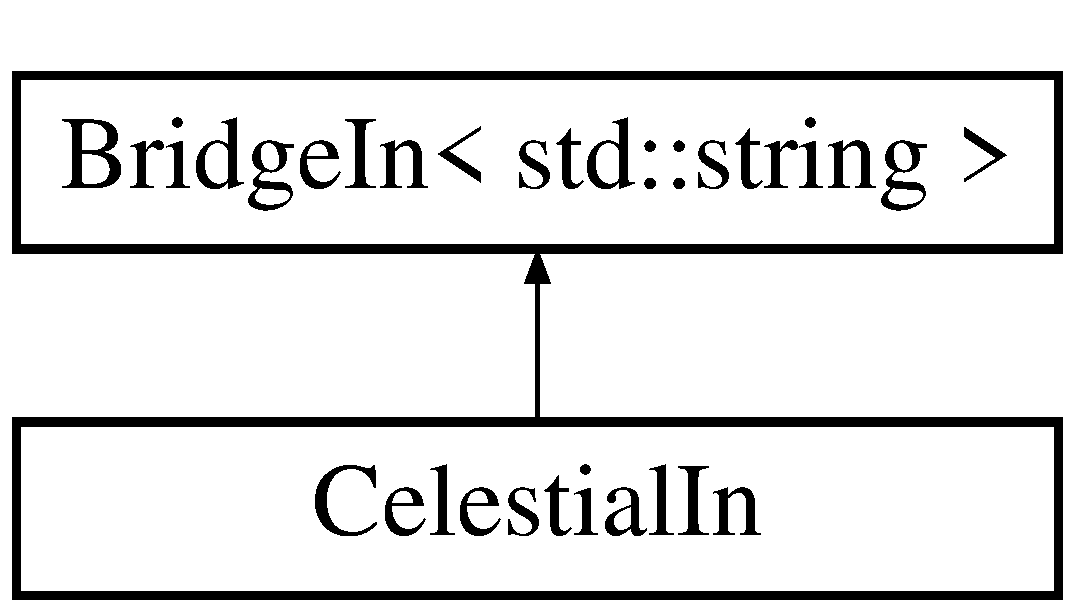
\includegraphics[height=2.000000cm]{classCelestialIn}
\end{center}
\end{figure}
\subsection*{Public Member Functions}
\begin{DoxyCompactItemize}
\item 
\mbox{\Hypertarget{classCelestialIn_a4d801ed723cdaefbfe60e9249558ce97}\label{classCelestialIn_a4d801ed723cdaefbfe60e9249558ce97}} 
{\bfseries Celestial\+In} (\mbox{\hyperlink{classTelescopeUI}{Telescope\+UI}} $\ast$const w)
\item 
\mbox{\Hypertarget{classCelestialIn_af0eebe637a588016616d4ded60c34ee8}\label{classCelestialIn_af0eebe637a588016616d4ded60c34ee8}} 
void {\bfseries slot} ()
\end{DoxyCompactItemize}
\subsection*{Additional Inherited Members}


The documentation for this class was generated from the following file\+:\begin{DoxyCompactItemize}
\item 
\mbox{\hyperlink{celestialin_8h}{celestialin.\+h}}\end{DoxyCompactItemize}

\hypertarget{classCelestialOut}{}\section{Celestial\+Out Class Reference}
\label{classCelestialOut}\index{Celestial\+Out@{Celestial\+Out}}
Inheritance diagram for Celestial\+Out\+:\begin{figure}[H]
\begin{center}
\leavevmode
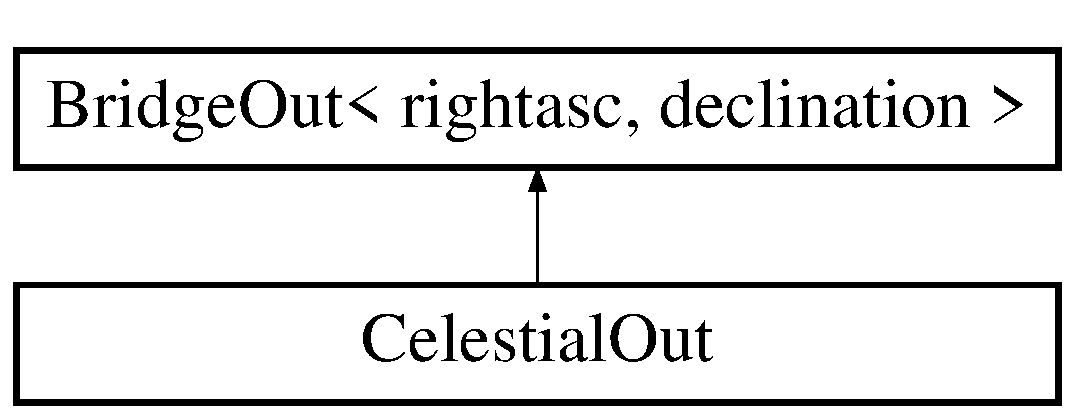
\includegraphics[height=2.000000cm]{classCelestialOut}
\end{center}
\end{figure}
\subsection*{Public Member Functions}
\begin{DoxyCompactItemize}
\item 
\mbox{\Hypertarget{classCelestialOut_a101fb3189ec42ef4f910db568b3e56a3}\label{classCelestialOut_a101fb3189ec42ef4f910db568b3e56a3}} 
{\bfseries Celestial\+Out} (\mbox{\hyperlink{structrightasc}{rightasc}} ra, \mbox{\hyperlink{structdeclination}{declination}} d)
\item 
\mbox{\Hypertarget{classCelestialOut_a47e713727665da513c6972da7657ccf2}\label{classCelestialOut_a47e713727665da513c6972da7657ccf2}} 
void {\bfseries update} ()
\end{DoxyCompactItemize}
\subsection*{Additional Inherited Members}


The documentation for this class was generated from the following file\+:\begin{DoxyCompactItemize}
\item 
celestialout.\+h\end{DoxyCompactItemize}

\hypertarget{classControlIn}{}\section{Control\+In Class Reference}
\label{classControlIn}\index{Control\+In@{Control\+In}}
Inheritance diagram for Control\+In\+:\begin{figure}[H]
\begin{center}
\leavevmode
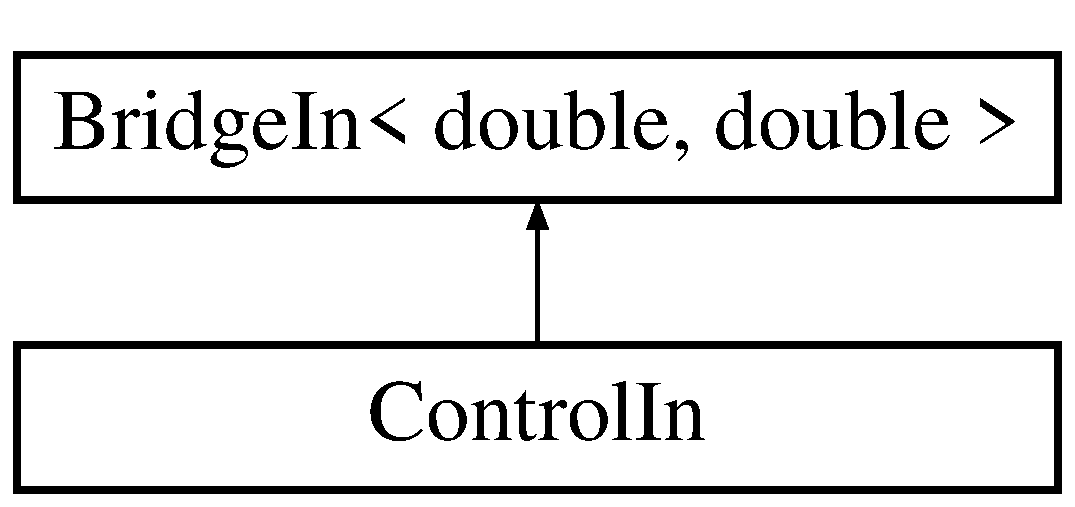
\includegraphics[height=2.000000cm]{classControlIn}
\end{center}
\end{figure}
\subsection*{Public Member Functions}
\begin{DoxyCompactItemize}
\item 
\mbox{\Hypertarget{classControlIn_aadc5715e6adde869b3887a6e12568364}\label{classControlIn_aadc5715e6adde869b3887a6e12568364}} 
{\bfseries Control\+In} (\mbox{\hyperlink{classTelescopeUI}{Telescope\+UI}} $\ast$const w)
\item 
\mbox{\Hypertarget{classControlIn_a4c412fb7e8009e94234487106fa605a5}\label{classControlIn_a4c412fb7e8009e94234487106fa605a5}} 
void {\bfseries slot} ()
\end{DoxyCompactItemize}
\subsection*{Additional Inherited Members}


The documentation for this class was generated from the following file\+:\begin{DoxyCompactItemize}
\item 
controlin.\+h\end{DoxyCompactItemize}

\hypertarget{classControlOut}{}\section{Control\+Out Class Reference}
\label{classControlOut}\index{Control\+Out@{Control\+Out}}
Inheritance diagram for Control\+Out\+:\begin{figure}[H]
\begin{center}
\leavevmode
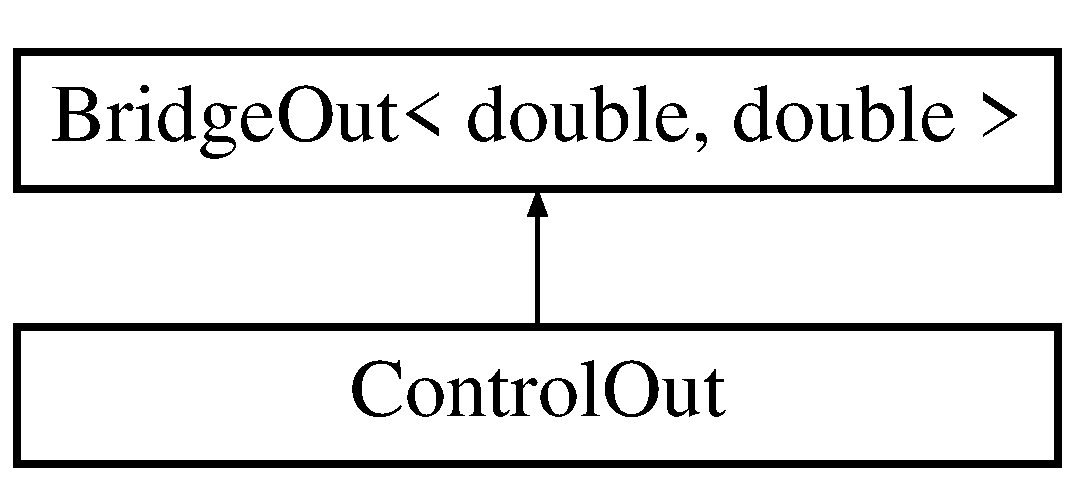
\includegraphics[height=2.000000cm]{classControlOut}
\end{center}
\end{figure}
\subsection*{Public Member Functions}
\begin{DoxyCompactItemize}
\item 
\mbox{\Hypertarget{classControlOut_a1736a35a73cb181610c72ced146cc500}\label{classControlOut_a1736a35a73cb181610c72ced146cc500}} 
{\bfseries Control\+Out} (double yaw\+\_\+value, double pitch\+\_\+value)
\item 
\mbox{\Hypertarget{classControlOut_ae7753a9f60e8574ed8c8bb5afae28a03}\label{classControlOut_ae7753a9f60e8574ed8c8bb5afae28a03}} 
void {\bfseries update} ()
\end{DoxyCompactItemize}
\subsection*{Additional Inherited Members}


The documentation for this class was generated from the following file\+:\begin{DoxyCompactItemize}
\item 
controlout.\+h\end{DoxyCompactItemize}

\hypertarget{structdeclination}{}\section{declination Struct Reference}
\label{structdeclination}\index{declination@{declination}}
\subsection*{Public Attributes}
\begin{DoxyCompactItemize}
\item 
\mbox{\Hypertarget{structdeclination_a6d57698dc945a9e462acd901876eacbe}\label{structdeclination_a6d57698dc945a9e462acd901876eacbe}} 
int {\bfseries d}
\item 
\mbox{\Hypertarget{structdeclination_a831039a43f7b7d21fb5e940a5e4d3c37}\label{structdeclination_a831039a43f7b7d21fb5e940a5e4d3c37}} 
int {\bfseries am}
\item 
\mbox{\Hypertarget{structdeclination_a724a25c740ad71b350915545f0d20934}\label{structdeclination_a724a25c740ad71b350915545f0d20934}} 
double {\bfseries as}
\end{DoxyCompactItemize}


The documentation for this struct was generated from the following file\+:\begin{DoxyCompactItemize}
\item 
\mbox{\hyperlink{coordinates_8h}{coordinates.\+h}}\end{DoxyCompactItemize}

\hypertarget{classEquatorialCoordinates}{}\section{Equatorial\+Coordinates Class Reference}
\label{classEquatorialCoordinates}\index{Equatorial\+Coordinates@{Equatorial\+Coordinates}}
\subsection*{Public Member Functions}
\begin{DoxyCompactItemize}
\item 
\mbox{\hyperlink{classEquatorialCoordinates_a4a147efb5882e12d1f8bc5cacd0e51a7}{Equatorial\+Coordinates}} (\mbox{\hyperlink{classAngle}{Angle}} right\+\_\+ascension, \mbox{\hyperlink{classAngle}{Angle}} \mbox{\hyperlink{structdeclination}{declination}})
\begin{DoxyCompactList}\small\item\em constructor method for \mbox{\hyperlink{classEquatorialCoordinates}{Equatorial\+Coordinates}} using right ascension and declination Angles \end{DoxyCompactList}\item 
\mbox{\hyperlink{classAngle}{Angle}} \mbox{\hyperlink{classEquatorialCoordinates_a48517346b93fc6b7082ebaed0851a6e8}{get\+\_\+right\+\_\+ascension}} ()
\begin{DoxyCompactList}\small\item\em getter method for the right ascension \end{DoxyCompactList}\item 
void \mbox{\hyperlink{classEquatorialCoordinates_ad6eac3da25d92a4e6c52f920d825ed43}{set\+\_\+right\+\_\+ascension}} (\mbox{\hyperlink{classAngle}{Angle}} right\+\_\+ascension)
\begin{DoxyCompactList}\small\item\em setter method for the right ascension \end{DoxyCompactList}\item 
\mbox{\hyperlink{classAngle}{Angle}} \mbox{\hyperlink{classEquatorialCoordinates_abdfc3d2ece63332b9a6a2267ae886710}{get\+\_\+declination}} ()
\begin{DoxyCompactList}\small\item\em getter method for the declination \end{DoxyCompactList}\item 
void \mbox{\hyperlink{classEquatorialCoordinates_ad3136302cdf4904010f22407071aa722}{set\+\_\+declination}} (\mbox{\hyperlink{classAngle}{Angle}} \mbox{\hyperlink{structdeclination}{declination}})
\begin{DoxyCompactList}\small\item\em setter method for the declination \end{DoxyCompactList}\item 
\mbox{\hyperlink{classHorizontalCoordinates}{Horizontal\+Coordinates}} \mbox{\hyperlink{classEquatorialCoordinates_a8e829ee947df5d5d823c4a25417de75c}{get\+\_\+horizontal}} (\mbox{\hyperlink{classAngle}{Angle}} latitude, \mbox{\hyperlink{classAngle}{Angle}} longitude, \mbox{\hyperlink{classAngle}{Angle}} local\+\_\+sidereal\+\_\+time)
\begin{DoxyCompactList}\small\item\em convert coordinates to the horizontal system (see\+: \href{http://star-www.st-and.ac.uk/~fv/webnotes/chapter7.htm}{\tt http\+://star-\/www.\+st-\/and.\+ac.\+uk/$\sim$fv/webnotes/chapter7.\+htm} ) \end{DoxyCompactList}\end{DoxyCompactItemize}
\subsection*{Private Attributes}
\begin{DoxyCompactItemize}
\item 
\mbox{\Hypertarget{classEquatorialCoordinates_ac8567b85d8e8818a44882198e2cac54c}\label{classEquatorialCoordinates_ac8567b85d8e8818a44882198e2cac54c}} 
\mbox{\hyperlink{classAngle}{Angle}} \mbox{\hyperlink{classEquatorialCoordinates_ac8567b85d8e8818a44882198e2cac54c}{\+\_\+right\+\_\+ascension}}
\begin{DoxyCompactList}\small\item\em internal representation of the right ascension \end{DoxyCompactList}\item 
\mbox{\Hypertarget{classEquatorialCoordinates_a424d605f2710fd158602b800e77a9882}\label{classEquatorialCoordinates_a424d605f2710fd158602b800e77a9882}} 
\mbox{\hyperlink{classAngle}{Angle}} \mbox{\hyperlink{classEquatorialCoordinates_a424d605f2710fd158602b800e77a9882}{\+\_\+declination}}
\begin{DoxyCompactList}\small\item\em internal representation of the declination \end{DoxyCompactList}\end{DoxyCompactItemize}


\subsection{Constructor \& Destructor Documentation}
\mbox{\Hypertarget{classEquatorialCoordinates_a4a147efb5882e12d1f8bc5cacd0e51a7}\label{classEquatorialCoordinates_a4a147efb5882e12d1f8bc5cacd0e51a7}} 
\index{Equatorial\+Coordinates@{Equatorial\+Coordinates}!Equatorial\+Coordinates@{Equatorial\+Coordinates}}
\index{Equatorial\+Coordinates@{Equatorial\+Coordinates}!Equatorial\+Coordinates@{Equatorial\+Coordinates}}
\subsubsection{\texorpdfstring{Equatorial\+Coordinates()}{EquatorialCoordinates()}}
{\footnotesize\ttfamily Equatorial\+Coordinates\+::\+Equatorial\+Coordinates (\begin{DoxyParamCaption}\item[{\mbox{\hyperlink{classAngle}{Angle}}}]{right\+\_\+ascension,  }\item[{\mbox{\hyperlink{classAngle}{Angle}}}]{declination }\end{DoxyParamCaption})}



constructor method for \mbox{\hyperlink{classEquatorialCoordinates}{Equatorial\+Coordinates}} using right ascension and declination Angles 


\begin{DoxyParams}{Parameters}
{\em altitude} & right\+\_\+ascension the altitude right ascension as an \mbox{\hyperlink{classAngle}{Angle}} \\
\hline
{\em declination} & represents the declination component as an \mbox{\hyperlink{classAngle}{Angle}} \\
\hline
\end{DoxyParams}


\subsection{Member Function Documentation}
\mbox{\Hypertarget{classEquatorialCoordinates_abdfc3d2ece63332b9a6a2267ae886710}\label{classEquatorialCoordinates_abdfc3d2ece63332b9a6a2267ae886710}} 
\index{Equatorial\+Coordinates@{Equatorial\+Coordinates}!get\+\_\+declination@{get\+\_\+declination}}
\index{get\+\_\+declination@{get\+\_\+declination}!Equatorial\+Coordinates@{Equatorial\+Coordinates}}
\subsubsection{\texorpdfstring{get\+\_\+declination()}{get\_declination()}}
{\footnotesize\ttfamily \mbox{\hyperlink{classAngle}{Angle}} Equatorial\+Coordinates\+::get\+\_\+declination (\begin{DoxyParamCaption}{ }\end{DoxyParamCaption})}



getter method for the declination 

\begin{DoxyReturn}{Returns}
the declination as an \mbox{\hyperlink{classAngle}{Angle}} 
\end{DoxyReturn}
\mbox{\Hypertarget{classEquatorialCoordinates_a8e829ee947df5d5d823c4a25417de75c}\label{classEquatorialCoordinates_a8e829ee947df5d5d823c4a25417de75c}} 
\index{Equatorial\+Coordinates@{Equatorial\+Coordinates}!get\+\_\+horizontal@{get\+\_\+horizontal}}
\index{get\+\_\+horizontal@{get\+\_\+horizontal}!Equatorial\+Coordinates@{Equatorial\+Coordinates}}
\subsubsection{\texorpdfstring{get\+\_\+horizontal()}{get\_horizontal()}}
{\footnotesize\ttfamily \mbox{\hyperlink{classHorizontalCoordinates}{Horizontal\+Coordinates}} Equatorial\+Coordinates\+::get\+\_\+horizontal (\begin{DoxyParamCaption}\item[{\mbox{\hyperlink{classAngle}{Angle}}}]{latitude,  }\item[{\mbox{\hyperlink{classAngle}{Angle}}}]{longitude,  }\item[{\mbox{\hyperlink{classAngle}{Angle}}}]{local\+\_\+sidereal\+\_\+time }\end{DoxyParamCaption})}



convert coordinates to the horizontal system (see\+: \href{http://star-www.st-and.ac.uk/~fv/webnotes/chapter7.htm}{\tt http\+://star-\/www.\+st-\/and.\+ac.\+uk/$\sim$fv/webnotes/chapter7.\+htm} ) 


\begin{DoxyParams}{Parameters}
{\em latitude} & represents the user\textquotesingle{}s latitude as an \mbox{\hyperlink{classAngle}{Angle}} \\
\hline
{\em longitude} & represents the user\textquotesingle{}s longitude as an \mbox{\hyperlink{classAngle}{Angle}} \\
\hline
{\em local\+\_\+sidereal\+\_\+time} & represents the current local sidereal time as an \mbox{\hyperlink{classAngle}{Angle}} \\
\hline
\end{DoxyParams}
\begin{DoxyReturn}{Returns}
the same celestial coordinates, represented in the horizontal system 
\end{DoxyReturn}
\mbox{\Hypertarget{classEquatorialCoordinates_a48517346b93fc6b7082ebaed0851a6e8}\label{classEquatorialCoordinates_a48517346b93fc6b7082ebaed0851a6e8}} 
\index{Equatorial\+Coordinates@{Equatorial\+Coordinates}!get\+\_\+right\+\_\+ascension@{get\+\_\+right\+\_\+ascension}}
\index{get\+\_\+right\+\_\+ascension@{get\+\_\+right\+\_\+ascension}!Equatorial\+Coordinates@{Equatorial\+Coordinates}}
\subsubsection{\texorpdfstring{get\+\_\+right\+\_\+ascension()}{get\_right\_ascension()}}
{\footnotesize\ttfamily \mbox{\hyperlink{classAngle}{Angle}} Equatorial\+Coordinates\+::get\+\_\+right\+\_\+ascension (\begin{DoxyParamCaption}{ }\end{DoxyParamCaption})}



getter method for the right ascension 

\begin{DoxyReturn}{Returns}
the right ascension as an \mbox{\hyperlink{classAngle}{Angle}} 
\end{DoxyReturn}
\mbox{\Hypertarget{classEquatorialCoordinates_ad3136302cdf4904010f22407071aa722}\label{classEquatorialCoordinates_ad3136302cdf4904010f22407071aa722}} 
\index{Equatorial\+Coordinates@{Equatorial\+Coordinates}!set\+\_\+declination@{set\+\_\+declination}}
\index{set\+\_\+declination@{set\+\_\+declination}!Equatorial\+Coordinates@{Equatorial\+Coordinates}}
\subsubsection{\texorpdfstring{set\+\_\+declination()}{set\_declination()}}
{\footnotesize\ttfamily void Equatorial\+Coordinates\+::set\+\_\+declination (\begin{DoxyParamCaption}\item[{\mbox{\hyperlink{classAngle}{Angle}}}]{declination }\end{DoxyParamCaption})}



setter method for the declination 


\begin{DoxyParams}{Parameters}
{\em declination} & represents the declination as an \mbox{\hyperlink{classAngle}{Angle}} \\
\hline
\end{DoxyParams}
\mbox{\Hypertarget{classEquatorialCoordinates_ad6eac3da25d92a4e6c52f920d825ed43}\label{classEquatorialCoordinates_ad6eac3da25d92a4e6c52f920d825ed43}} 
\index{Equatorial\+Coordinates@{Equatorial\+Coordinates}!set\+\_\+right\+\_\+ascension@{set\+\_\+right\+\_\+ascension}}
\index{set\+\_\+right\+\_\+ascension@{set\+\_\+right\+\_\+ascension}!Equatorial\+Coordinates@{Equatorial\+Coordinates}}
\subsubsection{\texorpdfstring{set\+\_\+right\+\_\+ascension()}{set\_right\_ascension()}}
{\footnotesize\ttfamily void Equatorial\+Coordinates\+::set\+\_\+right\+\_\+ascension (\begin{DoxyParamCaption}\item[{\mbox{\hyperlink{classAngle}{Angle}}}]{right\+\_\+ascension }\end{DoxyParamCaption})}



setter method for the right ascension 


\begin{DoxyParams}{Parameters}
{\em right\+\_\+ascension} & represents the right ascension as an \mbox{\hyperlink{classAngle}{Angle}} \\
\hline
\end{DoxyParams}


The documentation for this class was generated from the following files\+:\begin{DoxyCompactItemize}
\item 
\mbox{\hyperlink{EquatorialCoordinates_8h}{Equatorial\+Coordinates.\+h}}\item 
Equatorial\+Coordinates.\+cpp\end{DoxyCompactItemize}

\hypertarget{structFakeSerial}{}\section{Fake\+Serial Class Reference}
\label{structFakeSerial}\index{Fake\+Serial@{Fake\+Serial}}
\subsection*{Public Member Functions}
\begin{DoxyCompactItemize}
\item 
\mbox{\Hypertarget{structFakeSerial_a63a10269c62490d9a3406e086b70d035}\label{structFakeSerial_a63a10269c62490d9a3406e086b70d035}} 
{\bfseries Fake\+Serial} (\mbox{\hyperlink{structFakeSerial}{Fake\+Serial}} const \&)=delete
\item 
\mbox{\Hypertarget{structFakeSerial_ab7554e211e435a9079d4395486eb6f9e}\label{structFakeSerial_ab7554e211e435a9079d4395486eb6f9e}} 
void {\bfseries operator=} (\mbox{\hyperlink{structFakeSerial}{Fake\+Serial}} const \&)=delete
\item 
int \mbox{\hyperlink{structFakeSerial_ade2cc0ebb2014c45bdf2f5fb622da418}{read}} (char $\ast$buffer, unsigned int buf\+\_\+size)
\begin{DoxyCompactList}\small\item\em read the data from the arduino port \end{DoxyCompactList}\item 
bool \mbox{\hyperlink{structFakeSerial_ab25e13142d016f62831867434bcbd7cd}{write}} (char $\ast$buffer, unsigned int buf\+\_\+size)
\begin{DoxyCompactList}\small\item\em write the data into the arduio port \end{DoxyCompactList}\end{DoxyCompactItemize}
\subsection*{Private Attributes}
\begin{DoxyCompactItemize}
\item 
\mbox{\Hypertarget{structFakeSerial_a70ec5b8efe8fb0c15407db3c35732e6f}\label{structFakeSerial_a70ec5b8efe8fb0c15407db3c35732e6f}} 
double {\bfseries yaw}
\item 
\mbox{\Hypertarget{structFakeSerial_af5976686fbb6a720b9c15d9e3bd6a8c2}\label{structFakeSerial_af5976686fbb6a720b9c15d9e3bd6a8c2}} 
double {\bfseries pitch}
\end{DoxyCompactItemize}
\subsection*{Friends}
\begin{DoxyCompactItemize}
\item 
\mbox{\Hypertarget{structFakeSerial_abcbec8b664bd5afa556ae8ae6e8d1b8d}\label{structFakeSerial_abcbec8b664bd5afa556ae8ae6e8d1b8d}} 
\mbox{\hyperlink{structFakeSerial}{Fake\+Serial}} \& {\bfseries get\+\_\+test\+\_\+serial} ()
\end{DoxyCompactItemize}


\subsection{Member Function Documentation}
\mbox{\Hypertarget{structFakeSerial_ade2cc0ebb2014c45bdf2f5fb622da418}\label{structFakeSerial_ade2cc0ebb2014c45bdf2f5fb622da418}} 
\index{Fake\+Serial@{Fake\+Serial}!read@{read}}
\index{read@{read}!Fake\+Serial@{Fake\+Serial}}
\subsubsection{\texorpdfstring{read()}{read()}}
{\footnotesize\ttfamily int Fake\+Serial\+::read (\begin{DoxyParamCaption}\item[{char $\ast$}]{buffer,  }\item[{unsigned int}]{buf\+\_\+size }\end{DoxyParamCaption})}



read the data from the arduino port 


\begin{DoxyParams}{Parameters}
{\em buffer} & The data to read from the serial port \\
\hline
{\em buf\+\_\+size} & The size of the data buffer in bytes \\
\hline
\end{DoxyParams}
\begin{DoxyReturn}{Returns}
Integer representing the bytes that have been read in 
\end{DoxyReturn}
\mbox{\Hypertarget{structFakeSerial_ab25e13142d016f62831867434bcbd7cd}\label{structFakeSerial_ab25e13142d016f62831867434bcbd7cd}} 
\index{Fake\+Serial@{Fake\+Serial}!write@{write}}
\index{write@{write}!Fake\+Serial@{Fake\+Serial}}
\subsubsection{\texorpdfstring{write()}{write()}}
{\footnotesize\ttfamily bool Fake\+Serial\+::write (\begin{DoxyParamCaption}\item[{char $\ast$}]{buffer,  }\item[{unsigned int}]{buf\+\_\+size }\end{DoxyParamCaption})}



write the data into the arduio port 


\begin{DoxyParams}{Parameters}
{\em buffer} & The data to write into the serial port \\
\hline
{\em buf\+\_\+size} & The size of the data buffer in bytes \\
\hline
\end{DoxyParams}
\begin{DoxyReturn}{Returns}
Whether the write is successful (true) or not (false) 
\end{DoxyReturn}


The documentation for this class was generated from the following files\+:\begin{DoxyCompactItemize}
\item 
\mbox{\hyperlink{fakeserial_8h}{fakeserial.\+h}}\item 
fakeserial.\+cpp\end{DoxyCompactItemize}

\hypertarget{classFullStepController}{}\section{Full\+Step\+Controller Class Reference}
\label{classFullStepController}\index{Full\+Step\+Controller@{Full\+Step\+Controller}}
\subsection*{Public Member Functions}
\begin{DoxyCompactItemize}
\item 
\mbox{\Hypertarget{classFullStepController_acf4f6bac31f4cf72b16198b09f39600d}\label{classFullStepController_acf4f6bac31f4cf72b16198b09f39600d}} 
{\bfseries Full\+Step\+Controller} (unsigned int steps\+\_\+per\+\_\+rotation, unsigned int step\+\_\+period, unsigned int step\+\_\+pin, unsigned int dir\+\_\+pin)
\item 
\mbox{\Hypertarget{classFullStepController_a9dcb8326026c99fef86d14c73abfb46a}\label{classFullStepController_a9dcb8326026c99fef86d14c73abfb46a}} 
unsigned int {\bfseries step\+\_\+cw} ()
\item 
\mbox{\Hypertarget{classFullStepController_a1704b0c470b806ace4d9ceecb0cef8ef}\label{classFullStepController_a1704b0c470b806ace4d9ceecb0cef8ef}} 
unsigned int {\bfseries step\+\_\+ccw} ()
\item 
\mbox{\Hypertarget{classFullStepController_a24868fd43d69b51b3189449d11c23dc6}\label{classFullStepController_a24868fd43d69b51b3189449d11c23dc6}} 
unsigned int {\bfseries run\+\_\+by} (unsigned int n\+\_\+steps)
\item 
\mbox{\Hypertarget{classFullStepController_a4d17cf50e94538af8e9c1c55f75a2972}\label{classFullStepController_a4d17cf50e94538af8e9c1c55f75a2972}} 
unsigned int {\bfseries floor\+\_\+run} (double angle)
\item 
\mbox{\Hypertarget{classFullStepController_af6315b258390ca186a47a03ed6e961ec}\label{classFullStepController_af6315b258390ca186a47a03ed6e961ec}} 
unsigned int {\bfseries ceil\+\_\+run} (double angle)
\item 
\mbox{\Hypertarget{classFullStepController_ac0d4ed7da3364dfe9bf575a07c7cf9c5}\label{classFullStepController_ac0d4ed7da3364dfe9bf575a07c7cf9c5}} 
unsigned int {\bfseries get\+\_\+step\+\_\+period} ()
\item 
\mbox{\Hypertarget{classFullStepController_acc4af90ef8aa84618ebc6c9ba8f5b6eb}\label{classFullStepController_acc4af90ef8aa84618ebc6c9ba8f5b6eb}} 
unsigned int {\bfseries get\+\_\+steps} ()
\item 
\mbox{\Hypertarget{classFullStepController_ac0bd6c53a259c542c33783b9246f381a}\label{classFullStepController_ac0bd6c53a259c542c33783b9246f381a}} 
double {\bfseries get\+\_\+angle} ()
\end{DoxyCompactItemize}
\subsection*{Private Attributes}
\begin{DoxyCompactItemize}
\item 
\mbox{\Hypertarget{classFullStepController_afc92f9d012da060b6b9be7a670fb9878}\label{classFullStepController_afc92f9d012da060b6b9be7a670fb9878}} 
unsigned int {\bfseries step\+\_\+period}
\item 
\mbox{\Hypertarget{classFullStepController_abbf462dac01856f90aeb3ef0f2cf0b3e}\label{classFullStepController_abbf462dac01856f90aeb3ef0f2cf0b3e}} 
unsigned int {\bfseries step\+\_\+pin}
\item 
\mbox{\Hypertarget{classFullStepController_ab3f15365c34738b91161a672d3abc358}\label{classFullStepController_ab3f15365c34738b91161a672d3abc358}} 
unsigned int {\bfseries dir\+\_\+pin}
\item 
\mbox{\Hypertarget{classFullStepController_a13c27cad1a8401ca9a8c6829deb8194d}\label{classFullStepController_a13c27cad1a8401ca9a8c6829deb8194d}} 
\mbox{\hyperlink{classStepper}{Stepper}} {\bfseries stepper}
\end{DoxyCompactItemize}


The documentation for this class was generated from the following files\+:\begin{DoxyCompactItemize}
\item 
\mbox{\hyperlink{FullStepController_8h}{Full\+Step\+Controller.\+h}}\item 
Full\+Step\+Controller.\+cpp\end{DoxyCompactItemize}

\hypertarget{classHorizontalCoordinates}{}\section{Horizontal\+Coordinates Class Reference}
\label{classHorizontalCoordinates}\index{Horizontal\+Coordinates@{Horizontal\+Coordinates}}
\subsection*{Public Member Functions}
\begin{DoxyCompactItemize}
\item 
\mbox{\hyperlink{classHorizontalCoordinates_ac5b7b0e7f60d7fdb97b7a36c3adedfe3}{Horizontal\+Coordinates}} (\mbox{\hyperlink{classAngle}{Angle}} altitude, \mbox{\hyperlink{classAngle}{Angle}} azimuth)
\begin{DoxyCompactList}\small\item\em constructor method for \mbox{\hyperlink{classHorizontalCoordinates}{Horizontal\+Coordinates}} using altitude and azimuth Angles \end{DoxyCompactList}\item 
\mbox{\hyperlink{classAngle}{Angle}} \mbox{\hyperlink{classHorizontalCoordinates_a9c28aef9ec9276dea5d58fe5d8c4bece}{get\+\_\+altitude}} ()
\begin{DoxyCompactList}\small\item\em getter method for the altitude \end{DoxyCompactList}\item 
void \mbox{\hyperlink{classHorizontalCoordinates_a2112ee5b54653ca30712b7fa4a17482d}{set\+\_\+altitude}} (\mbox{\hyperlink{classAngle}{Angle}} altitude)
\begin{DoxyCompactList}\small\item\em setter method for the altitude \end{DoxyCompactList}\item 
\mbox{\hyperlink{classAngle}{Angle}} \mbox{\hyperlink{classHorizontalCoordinates_afb4b783738b13dbfb23035946c8a210d}{get\+\_\+azimuth}} ()
\begin{DoxyCompactList}\small\item\em getter method for the azimuth \end{DoxyCompactList}\item 
void \mbox{\hyperlink{classHorizontalCoordinates_a05fb79f9470d72b9e895c2cb7e10da94}{set\+\_\+azimuth}} (\mbox{\hyperlink{classAngle}{Angle}} azimuth)
\begin{DoxyCompactList}\small\item\em setter method for the azimuth \end{DoxyCompactList}\item 
\mbox{\hyperlink{classEquatorialCoordinates}{Equatorial\+Coordinates}} \mbox{\hyperlink{classHorizontalCoordinates_a1513f50fc1bdd2ded9934e783ada4e86}{get\+\_\+equatorial}} (\mbox{\hyperlink{classAngle}{Angle}} latitude, \mbox{\hyperlink{classAngle}{Angle}} longitude, \mbox{\hyperlink{classAngle}{Angle}} local\+\_\+sidereal\+\_\+time)
\begin{DoxyCompactList}\small\item\em convert coordinates to the equatorial system (see\+: \href{http://star-www.st-and.ac.uk/~fv/webnotes/chapter7.htm}{\tt http\+://star-\/www.\+st-\/and.\+ac.\+uk/$\sim$fv/webnotes/chapter7.\+htm} ) \end{DoxyCompactList}\end{DoxyCompactItemize}
\subsection*{Private Attributes}
\begin{DoxyCompactItemize}
\item 
\mbox{\Hypertarget{classHorizontalCoordinates_a4c31b8c5655757a613db12de45e275d2}\label{classHorizontalCoordinates_a4c31b8c5655757a613db12de45e275d2}} 
\mbox{\hyperlink{classAngle}{Angle}} \mbox{\hyperlink{classHorizontalCoordinates_a4c31b8c5655757a613db12de45e275d2}{\+\_\+altitude}}
\begin{DoxyCompactList}\small\item\em internal representation of the altitude \end{DoxyCompactList}\item 
\mbox{\Hypertarget{classHorizontalCoordinates_a4763500bc46d7b910fcb043b69bdc3d2}\label{classHorizontalCoordinates_a4763500bc46d7b910fcb043b69bdc3d2}} 
\mbox{\hyperlink{classAngle}{Angle}} \mbox{\hyperlink{classHorizontalCoordinates_a4763500bc46d7b910fcb043b69bdc3d2}{\+\_\+azimuth}}
\begin{DoxyCompactList}\small\item\em internal representation of the azimuth \end{DoxyCompactList}\end{DoxyCompactItemize}


\subsection{Constructor \& Destructor Documentation}
\mbox{\Hypertarget{classHorizontalCoordinates_ac5b7b0e7f60d7fdb97b7a36c3adedfe3}\label{classHorizontalCoordinates_ac5b7b0e7f60d7fdb97b7a36c3adedfe3}} 
\index{Horizontal\+Coordinates@{Horizontal\+Coordinates}!Horizontal\+Coordinates@{Horizontal\+Coordinates}}
\index{Horizontal\+Coordinates@{Horizontal\+Coordinates}!Horizontal\+Coordinates@{Horizontal\+Coordinates}}
\subsubsection{\texorpdfstring{Horizontal\+Coordinates()}{HorizontalCoordinates()}}
{\footnotesize\ttfamily Horizontal\+Coordinates\+::\+Horizontal\+Coordinates (\begin{DoxyParamCaption}\item[{\mbox{\hyperlink{classAngle}{Angle}}}]{altitude,  }\item[{\mbox{\hyperlink{classAngle}{Angle}}}]{azimuth }\end{DoxyParamCaption})}



constructor method for \mbox{\hyperlink{classHorizontalCoordinates}{Horizontal\+Coordinates}} using altitude and azimuth Angles 


\begin{DoxyParams}{Parameters}
{\em altitude} & represents the altitude component as an \mbox{\hyperlink{classAngle}{Angle}} \\
\hline
{\em azimuth} & represents the azimuth component as an \mbox{\hyperlink{classAngle}{Angle}} \\
\hline
\end{DoxyParams}


\subsection{Member Function Documentation}
\mbox{\Hypertarget{classHorizontalCoordinates_a9c28aef9ec9276dea5d58fe5d8c4bece}\label{classHorizontalCoordinates_a9c28aef9ec9276dea5d58fe5d8c4bece}} 
\index{Horizontal\+Coordinates@{Horizontal\+Coordinates}!get\+\_\+altitude@{get\+\_\+altitude}}
\index{get\+\_\+altitude@{get\+\_\+altitude}!Horizontal\+Coordinates@{Horizontal\+Coordinates}}
\subsubsection{\texorpdfstring{get\+\_\+altitude()}{get\_altitude()}}
{\footnotesize\ttfamily \mbox{\hyperlink{classAngle}{Angle}} Horizontal\+Coordinates\+::get\+\_\+altitude (\begin{DoxyParamCaption}{ }\end{DoxyParamCaption})}



getter method for the altitude 

\begin{DoxyReturn}{Returns}
the altitude as an \mbox{\hyperlink{classAngle}{Angle}} 
\end{DoxyReturn}
\mbox{\Hypertarget{classHorizontalCoordinates_afb4b783738b13dbfb23035946c8a210d}\label{classHorizontalCoordinates_afb4b783738b13dbfb23035946c8a210d}} 
\index{Horizontal\+Coordinates@{Horizontal\+Coordinates}!get\+\_\+azimuth@{get\+\_\+azimuth}}
\index{get\+\_\+azimuth@{get\+\_\+azimuth}!Horizontal\+Coordinates@{Horizontal\+Coordinates}}
\subsubsection{\texorpdfstring{get\+\_\+azimuth()}{get\_azimuth()}}
{\footnotesize\ttfamily \mbox{\hyperlink{classAngle}{Angle}} Horizontal\+Coordinates\+::get\+\_\+azimuth (\begin{DoxyParamCaption}{ }\end{DoxyParamCaption})}



getter method for the azimuth 

\begin{DoxyReturn}{Returns}
the azimuth as an \mbox{\hyperlink{classAngle}{Angle}} 
\end{DoxyReturn}
\mbox{\Hypertarget{classHorizontalCoordinates_a1513f50fc1bdd2ded9934e783ada4e86}\label{classHorizontalCoordinates_a1513f50fc1bdd2ded9934e783ada4e86}} 
\index{Horizontal\+Coordinates@{Horizontal\+Coordinates}!get\+\_\+equatorial@{get\+\_\+equatorial}}
\index{get\+\_\+equatorial@{get\+\_\+equatorial}!Horizontal\+Coordinates@{Horizontal\+Coordinates}}
\subsubsection{\texorpdfstring{get\+\_\+equatorial()}{get\_equatorial()}}
{\footnotesize\ttfamily \mbox{\hyperlink{classEquatorialCoordinates}{Equatorial\+Coordinates}} Horizontal\+Coordinates\+::get\+\_\+equatorial (\begin{DoxyParamCaption}\item[{\mbox{\hyperlink{classAngle}{Angle}}}]{latitude,  }\item[{\mbox{\hyperlink{classAngle}{Angle}}}]{longitude,  }\item[{\mbox{\hyperlink{classAngle}{Angle}}}]{local\+\_\+sidereal\+\_\+time }\end{DoxyParamCaption})}



convert coordinates to the equatorial system (see\+: \href{http://star-www.st-and.ac.uk/~fv/webnotes/chapter7.htm}{\tt http\+://star-\/www.\+st-\/and.\+ac.\+uk/$\sim$fv/webnotes/chapter7.\+htm} ) 


\begin{DoxyParams}{Parameters}
{\em latitude} & represents the user\textquotesingle{}s latitude as an \mbox{\hyperlink{classAngle}{Angle}} \\
\hline
{\em longitude} & represents the user\textquotesingle{}s longitude as an \mbox{\hyperlink{classAngle}{Angle}} \\
\hline
{\em local\+\_\+sidereal\+\_\+time} & represents the current local sidereal time as an \mbox{\hyperlink{classAngle}{Angle}} \\
\hline
\end{DoxyParams}
\begin{DoxyReturn}{Returns}
the same celestial coordinates, represented in the equatorial system 
\end{DoxyReturn}
\mbox{\Hypertarget{classHorizontalCoordinates_a2112ee5b54653ca30712b7fa4a17482d}\label{classHorizontalCoordinates_a2112ee5b54653ca30712b7fa4a17482d}} 
\index{Horizontal\+Coordinates@{Horizontal\+Coordinates}!set\+\_\+altitude@{set\+\_\+altitude}}
\index{set\+\_\+altitude@{set\+\_\+altitude}!Horizontal\+Coordinates@{Horizontal\+Coordinates}}
\subsubsection{\texorpdfstring{set\+\_\+altitude()}{set\_altitude()}}
{\footnotesize\ttfamily void Horizontal\+Coordinates\+::set\+\_\+altitude (\begin{DoxyParamCaption}\item[{\mbox{\hyperlink{classAngle}{Angle}}}]{altitude }\end{DoxyParamCaption})}



setter method for the altitude 


\begin{DoxyParams}{Parameters}
{\em altitude} & represents the altitude as an \mbox{\hyperlink{classAngle}{Angle}} \\
\hline
\end{DoxyParams}
\mbox{\Hypertarget{classHorizontalCoordinates_a05fb79f9470d72b9e895c2cb7e10da94}\label{classHorizontalCoordinates_a05fb79f9470d72b9e895c2cb7e10da94}} 
\index{Horizontal\+Coordinates@{Horizontal\+Coordinates}!set\+\_\+azimuth@{set\+\_\+azimuth}}
\index{set\+\_\+azimuth@{set\+\_\+azimuth}!Horizontal\+Coordinates@{Horizontal\+Coordinates}}
\subsubsection{\texorpdfstring{set\+\_\+azimuth()}{set\_azimuth()}}
{\footnotesize\ttfamily void Horizontal\+Coordinates\+::set\+\_\+azimuth (\begin{DoxyParamCaption}\item[{\mbox{\hyperlink{classAngle}{Angle}}}]{azimuth }\end{DoxyParamCaption})}



setter method for the azimuth 


\begin{DoxyParams}{Parameters}
{\em azimuth} & represents the altitude as an \mbox{\hyperlink{classAngle}{Angle}} \\
\hline
\end{DoxyParams}


The documentation for this class was generated from the following files\+:\begin{DoxyCompactItemize}
\item 
\mbox{\hyperlink{HorizontalCoordinates_8h}{Horizontal\+Coordinates.\+h}}\item 
\mbox{\hyperlink{HorizontalCoordinates_8cpp}{Horizontal\+Coordinates.\+cpp}}\end{DoxyCompactItemize}

\hypertarget{classManualTranslation}{}\section{Manual\+Translation Class Reference}
\label{classManualTranslation}\index{Manual\+Translation@{Manual\+Translation}}
\subsection*{Static Private Member Functions}
\begin{DoxyCompactItemize}
\item 
\mbox{\Hypertarget{classManualTranslation_a30730db174c38838524c5da363918df2}\label{classManualTranslation_a30730db174c38838524c5da363918df2}} 
static void {\bfseries to\+\_\+coords} (double yaw, double pitch)
\end{DoxyCompactItemize}


The documentation for this class was generated from the following file\+:\begin{DoxyCompactItemize}
\item 
translation.\+h\end{DoxyCompactItemize}

\hypertarget{structMotorControl}{}\section{Motor\+Control Class Reference}
\label{structMotorControl}\index{Motor\+Control@{Motor\+Control}}
\subsection*{Public Member Functions}
\begin{DoxyCompactItemize}
\item 
\mbox{\Hypertarget{structMotorControl_acaead1ae076590ce6a403658d94598ab}\label{structMotorControl_acaead1ae076590ce6a403658d94598ab}} 
{\bfseries Motor\+Control} (\mbox{\hyperlink{structMotorControl}{Motor\+Control}} const \&)=delete
\item 
\mbox{\Hypertarget{structMotorControl_a372ffb76326e3ac4fa825ed39536ee08}\label{structMotorControl_a372ffb76326e3ac4fa825ed39536ee08}} 
void {\bfseries operator=} (\mbox{\hyperlink{structMotorControl}{Motor\+Control}} const \&)=delete
\item 
std\+::pair$<$ double, double $>$ \mbox{\hyperlink{structMotorControl_ace9edcee1a69c1d56e2af842e2fd3b1a}{read\+\_\+pos}} ()
\begin{DoxyCompactList}\small\item\em returns the position read in from the serial port, doesn\textquotesingle{}t trigger any pins \end{DoxyCompactList}\item 
\mbox{\Hypertarget{structMotorControl_a16f947c331b12ae98e11f67ae1b4229d}\label{structMotorControl_a16f947c331b12ae98e11f67ae1b4229d}} 
void \mbox{\hyperlink{structMotorControl_a16f947c331b12ae98e11f67ae1b4229d}{all\+\_\+stop}} ()
\begin{DoxyCompactList}\small\item\em calls the all stop command by flipping the required pin to H\+I\+GH; this is blocking until activity pin is L\+OW \end{DoxyCompactList}\item 
bool \mbox{\hyperlink{structMotorControl_a2027a3374ee4ec606901c77931226e30}{write\+\_\+pos}} (double, double)
\begin{DoxyCompactList}\small\item\em writes the provided yaw and pitch to the serial port to give the motors a new direction, will not write if the resource is active \end{DoxyCompactList}\item 
bool \mbox{\hyperlink{structMotorControl_ae5ed3793c1b3e6f982bf6806ecce3978}{write\+\_\+vel}} (double, double)
\begin{DoxyCompactList}\small\item\em writes the provided yaw and pitch to the serial port to give the motors a new velocity, will not write if the resource is active \end{DoxyCompactList}\item 
bool \mbox{\hyperlink{structMotorControl_a9de35f14006d017df36b62d2c904249c}{is\+\_\+free}} ()
\begin{DoxyCompactList}\small\item\em returns whether the activity pin is H\+I\+GH or L\+OW \end{DoxyCompactList}\end{DoxyCompactItemize}
\subsection*{Static Public Member Functions}
\begin{DoxyCompactItemize}
\item 
\mbox{\Hypertarget{structMotorControl_a7c001c25110ea459918b239f0bbd5801}\label{structMotorControl_a7c001c25110ea459918b239f0bbd5801}} 
static \mbox{\hyperlink{structMotorControl}{Motor\+Control}} \& {\bfseries get\+\_\+instance} ()
\end{DoxyCompactItemize}
\subsection*{Private Attributes}
\begin{DoxyCompactItemize}
\item 
\mbox{\Hypertarget{structMotorControl_ac78d113a124d1de77371c77d7b52fc2f}\label{structMotorControl_ac78d113a124d1de77371c77d7b52fc2f}} 
\mbox{\hyperlink{classSerialPort}{Serial\+Port}} const {\bfseries serial}
\item 
\mbox{\Hypertarget{structMotorControl_ac0acc1ad145c1d1e30a8c335e537ae05}\label{structMotorControl_ac0acc1ad145c1d1e30a8c335e537ae05}} 
\mbox{\hyperlink{classPin}{Pin}} const {\bfseries ppos}
\item 
\mbox{\Hypertarget{structMotorControl_acd2298cf7680cb360aa15d5588ce41cb}\label{structMotorControl_acd2298cf7680cb360aa15d5588ce41cb}} 
\mbox{\hyperlink{classPin}{Pin}} const {\bfseries pvel}
\item 
\mbox{\Hypertarget{structMotorControl_aecda6adda398b0367f44c287cbe7311f}\label{structMotorControl_aecda6adda398b0367f44c287cbe7311f}} 
\mbox{\hyperlink{classPin}{Pin}} const {\bfseries pstate}
\item 
\mbox{\Hypertarget{structMotorControl_a9b9b48901301826eb2b2892c6967bc13}\label{structMotorControl_a9b9b48901301826eb2b2892c6967bc13}} 
\mbox{\hyperlink{classPin}{Pin}} const {\bfseries pstop}
\item 
\mbox{\Hypertarget{structMotorControl_a807d1fe97d6afc0ad367b5ed9c12a7e5}\label{structMotorControl_a807d1fe97d6afc0ad367b5ed9c12a7e5}} 
std\+::mutex {\bfseries mm}
\end{DoxyCompactItemize}
\subsection*{Friends}
\begin{DoxyCompactItemize}
\item 
\mbox{\Hypertarget{structMotorControl_a039b582e86435db0881e066f0b7a89b8}\label{structMotorControl_a039b582e86435db0881e066f0b7a89b8}} 
static friend \mbox{\hyperlink{structMotorControl}{Motor\+Control}} \& \mbox{\hyperlink{structMotorControl_a039b582e86435db0881e066f0b7a89b8}{motor\+\_\+driver}} ()
\begin{DoxyCompactList}\small\item\em let the motor driver function, which returns the state, easily access members from this class \end{DoxyCompactList}\end{DoxyCompactItemize}


\subsection{Member Function Documentation}
\mbox{\Hypertarget{structMotorControl_a9de35f14006d017df36b62d2c904249c}\label{structMotorControl_a9de35f14006d017df36b62d2c904249c}} 
\index{Motor\+Control@{Motor\+Control}!is\+\_\+free@{is\+\_\+free}}
\index{is\+\_\+free@{is\+\_\+free}!Motor\+Control@{Motor\+Control}}
\subsubsection{\texorpdfstring{is\+\_\+free()}{is\_free()}}
{\footnotesize\ttfamily bool Motor\+Control\+::is\+\_\+free (\begin{DoxyParamCaption}{ }\end{DoxyParamCaption})}



returns whether the activity pin is H\+I\+GH or L\+OW 

\begin{DoxyReturn}{Returns}
If the activity pin is H\+I\+GH then false, L\+OW then true 
\end{DoxyReturn}
\mbox{\Hypertarget{structMotorControl_ace9edcee1a69c1d56e2af842e2fd3b1a}\label{structMotorControl_ace9edcee1a69c1d56e2af842e2fd3b1a}} 
\index{Motor\+Control@{Motor\+Control}!read\+\_\+pos@{read\+\_\+pos}}
\index{read\+\_\+pos@{read\+\_\+pos}!Motor\+Control@{Motor\+Control}}
\subsubsection{\texorpdfstring{read\+\_\+pos()}{read\_pos()}}
{\footnotesize\ttfamily std\+::pair$<$ double, double $>$ Motor\+Control\+::read\+\_\+pos (\begin{DoxyParamCaption}{ }\end{DoxyParamCaption})}



returns the position read in from the serial port, doesn\textquotesingle{}t trigger any pins 

\begin{DoxyReturn}{Returns}
Pair object containing the yaw and pitch, respectively 
\end{DoxyReturn}
\mbox{\Hypertarget{structMotorControl_a2027a3374ee4ec606901c77931226e30}\label{structMotorControl_a2027a3374ee4ec606901c77931226e30}} 
\index{Motor\+Control@{Motor\+Control}!write\+\_\+pos@{write\+\_\+pos}}
\index{write\+\_\+pos@{write\+\_\+pos}!Motor\+Control@{Motor\+Control}}
\subsubsection{\texorpdfstring{write\+\_\+pos()}{write\_pos()}}
{\footnotesize\ttfamily bool Motor\+Control\+::write\+\_\+pos (\begin{DoxyParamCaption}\item[{double}]{yaw,  }\item[{double}]{pitch }\end{DoxyParamCaption})}



writes the provided yaw and pitch to the serial port to give the motors a new direction, will not write if the resource is active 


\begin{DoxyParams}{Parameters}
{\em yaw} & The new yaw position for the telescope \\
\hline
{\em pitch} & The new pitch position for the telescope \\
\hline
\end{DoxyParams}
\begin{DoxyReturn}{Returns}
Whether the write is successful (true) or not (false) 
\end{DoxyReturn}
\mbox{\Hypertarget{structMotorControl_ae5ed3793c1b3e6f982bf6806ecce3978}\label{structMotorControl_ae5ed3793c1b3e6f982bf6806ecce3978}} 
\index{Motor\+Control@{Motor\+Control}!write\+\_\+vel@{write\+\_\+vel}}
\index{write\+\_\+vel@{write\+\_\+vel}!Motor\+Control@{Motor\+Control}}
\subsubsection{\texorpdfstring{write\+\_\+vel()}{write\_vel()}}
{\footnotesize\ttfamily bool Motor\+Control\+::write\+\_\+vel (\begin{DoxyParamCaption}\item[{double}]{yaw,  }\item[{double}]{pitch }\end{DoxyParamCaption})}



writes the provided yaw and pitch to the serial port to give the motors a new velocity, will not write if the resource is active 


\begin{DoxyParams}{Parameters}
{\em yaw} & The new yaw velocity for the telescope \\
\hline
{\em pitch} & The new pitch velocity for the telescope \\
\hline
\end{DoxyParams}
\begin{DoxyReturn}{Returns}
Whether the write is successful (true) or not (false) 
\end{DoxyReturn}


The documentation for this class was generated from the following files\+:\begin{DoxyCompactItemize}
\item 
\mbox{\hyperlink{motorcontrol_8h}{motorcontrol.\+h}}\item 
motorcontrol.\+cpp\end{DoxyCompactItemize}

\hypertarget{classPin}{}\section{Pin Class Reference}
\label{classPin}\index{Pin@{Pin}}
\subsection*{Public Member Functions}
\begin{DoxyCompactItemize}
\item 
\mbox{\Hypertarget{classPin_aaf3d92065cd9b9de91f01164bec418ea}\label{classPin_aaf3d92065cd9b9de91f01164bec418ea}} 
\mbox{\hyperlink{classPin_aaf3d92065cd9b9de91f01164bec418ea}{Pin}} ()
\begin{DoxyCompactList}\small\item\em constructor, create a G\+P\+IO object and export \end{DoxyCompactList}\item 
\mbox{\hyperlink{classPin_a580d21a6d49bf1276146b0fab1a6039e}{Pin}} (int)
\begin{DoxyCompactList}\small\item\em constructor, export with the defined pin \end{DoxyCompactList}\item 
\mbox{\hyperlink{classPin_ae09bd2322f5ebbfaf98a379566d88ac0}{Pin}} (int, char $\ast$)
\begin{DoxyCompactList}\small\item\em constructor, give the direction of the pin too \end{DoxyCompactList}\item 
\mbox{\Hypertarget{classPin_a462c14c45d3d653731dde638aa6e7bb7}\label{classPin_a462c14c45d3d653731dde638aa6e7bb7}} 
\mbox{\hyperlink{classPin_a462c14c45d3d653731dde638aa6e7bb7}{$\sim$\+Pin}} ()
\begin{DoxyCompactList}\small\item\em destructor, exports the pin \end{DoxyCompactList}\item 
int \mbox{\hyperlink{classPin_a233ab381d3ebab706ca96bc3b78f0927}{export\+\_\+gpio}} ()
\begin{DoxyCompactList}\small\item\em exports G\+P\+IO \end{DoxyCompactList}\item 
int \mbox{\hyperlink{classPin_ac0010e89c86e30b5e453f223ec591e1f}{unexport\+\_\+gpio}} ()
\begin{DoxyCompactList}\small\item\em exports G\+P\+IO \end{DoxyCompactList}\item 
int \mbox{\hyperlink{classPin_a40c6f300d3c97b653fb598ca36a8d778}{setdir\+\_\+gpio}} (char $\ast$dir)
\begin{DoxyCompactList}\small\item\em sets the direction of G\+P\+IO pin, should only be called once \end{DoxyCompactList}\item 
int \mbox{\hyperlink{classPin_a319c0b85b6b667b6708fe501a47c061c}{setval\+\_\+gpio}} (int val) const
\begin{DoxyCompactList}\small\item\em sets a new value for G\+P\+IO pin \end{DoxyCompactList}\item 
int \mbox{\hyperlink{classPin_a04fc4921bf674049be0d06842709913f}{getval\+\_\+gpio}} (int \&val) const
\begin{DoxyCompactList}\small\item\em gets G\+P\+IO value \end{DoxyCompactList}\item 
int \mbox{\hyperlink{classPin_a180d487895b4fc270437af97a0428f22}{get\+\_\+gpionum}} () const
\begin{DoxyCompactList}\small\item\em gets G\+P\+IO pin number \end{DoxyCompactList}\end{DoxyCompactItemize}
\subsection*{Private Member Functions}
\begin{DoxyCompactItemize}
\item 
int \mbox{\hyperlink{classPin_a1ab3312c109c400607d3242f0463941b}{write}} (char $\ast$to, char $\ast$val) const
\begin{DoxyCompactList}\small\item\em writes the asked value to the asked directory \end{DoxyCompactList}\item 
int \mbox{\hyperlink{classPin_a800322aedd71b00ea963876b6628be68}{write}} (char $\ast$to, int val) const
\begin{DoxyCompactList}\small\item\em writes the asked value to the asked directory \end{DoxyCompactList}\end{DoxyCompactItemize}
\subsection*{Private Attributes}
\begin{DoxyCompactItemize}
\item 
\mbox{\Hypertarget{classPin_a1e8d9e0fd44e407c7a4ebcfa7f72e199}\label{classPin_a1e8d9e0fd44e407c7a4ebcfa7f72e199}} 
int const {\bfseries gpionum}
\end{DoxyCompactItemize}


\subsection{Constructor \& Destructor Documentation}
\mbox{\Hypertarget{classPin_a580d21a6d49bf1276146b0fab1a6039e}\label{classPin_a580d21a6d49bf1276146b0fab1a6039e}} 
\index{Pin@{Pin}!Pin@{Pin}}
\index{Pin@{Pin}!Pin@{Pin}}
\subsubsection{\texorpdfstring{Pin()}{Pin()}\hspace{0.1cm}{\footnotesize\ttfamily [1/2]}}
{\footnotesize\ttfamily Pin\+::\+Pin (\begin{DoxyParamCaption}\item[{int}]{gpionum }\end{DoxyParamCaption})}



constructor, export with the defined pin 


\begin{DoxyParams}{Parameters}
{\em gpionum} & The pin number for this pin \\
\hline
\end{DoxyParams}
\mbox{\Hypertarget{classPin_ae09bd2322f5ebbfaf98a379566d88ac0}\label{classPin_ae09bd2322f5ebbfaf98a379566d88ac0}} 
\index{Pin@{Pin}!Pin@{Pin}}
\index{Pin@{Pin}!Pin@{Pin}}
\subsubsection{\texorpdfstring{Pin()}{Pin()}\hspace{0.1cm}{\footnotesize\ttfamily [2/2]}}
{\footnotesize\ttfamily Pin\+::\+Pin (\begin{DoxyParamCaption}\item[{int}]{gpionum,  }\item[{char $\ast$}]{dir }\end{DoxyParamCaption})}



constructor, give the direction of the pin too 


\begin{DoxyParams}{Parameters}
{\em gpionum} & The pin number for this pin \\
\hline
{\em dir} & The direction for this pin \\
\hline
\end{DoxyParams}


\subsection{Member Function Documentation}
\mbox{\Hypertarget{classPin_a233ab381d3ebab706ca96bc3b78f0927}\label{classPin_a233ab381d3ebab706ca96bc3b78f0927}} 
\index{Pin@{Pin}!export\+\_\+gpio@{export\+\_\+gpio}}
\index{export\+\_\+gpio@{export\+\_\+gpio}!Pin@{Pin}}
\subsubsection{\texorpdfstring{export\+\_\+gpio()}{export\_gpio()}}
{\footnotesize\ttfamily int Pin\+::export\+\_\+gpio (\begin{DoxyParamCaption}{ }\end{DoxyParamCaption})}



exports G\+P\+IO 

\begin{DoxyReturn}{Returns}
Whether the export succeeded (1) or failed (0) 
\end{DoxyReturn}
\mbox{\Hypertarget{classPin_a180d487895b4fc270437af97a0428f22}\label{classPin_a180d487895b4fc270437af97a0428f22}} 
\index{Pin@{Pin}!get\+\_\+gpionum@{get\+\_\+gpionum}}
\index{get\+\_\+gpionum@{get\+\_\+gpionum}!Pin@{Pin}}
\subsubsection{\texorpdfstring{get\+\_\+gpionum()}{get\_gpionum()}}
{\footnotesize\ttfamily int Pin\+::get\+\_\+gpionum (\begin{DoxyParamCaption}{ }\end{DoxyParamCaption}) const}



gets G\+P\+IO pin number 

\begin{DoxyReturn}{Returns}
The pin number 
\end{DoxyReturn}
\mbox{\Hypertarget{classPin_a04fc4921bf674049be0d06842709913f}\label{classPin_a04fc4921bf674049be0d06842709913f}} 
\index{Pin@{Pin}!getval\+\_\+gpio@{getval\+\_\+gpio}}
\index{getval\+\_\+gpio@{getval\+\_\+gpio}!Pin@{Pin}}
\subsubsection{\texorpdfstring{getval\+\_\+gpio()}{getval\_gpio()}}
{\footnotesize\ttfamily int Pin\+::getval\+\_\+gpio (\begin{DoxyParamCaption}\item[{int \&}]{val }\end{DoxyParamCaption}) const}



gets G\+P\+IO value 


\begin{DoxyParams}{Parameters}
{\em value} & The integer to print the output to \\
\hline
\end{DoxyParams}
\begin{DoxyReturn}{Returns}
Whether the get succeeded (1) or failed (0) 
\end{DoxyReturn}
\mbox{\Hypertarget{classPin_a40c6f300d3c97b653fb598ca36a8d778}\label{classPin_a40c6f300d3c97b653fb598ca36a8d778}} 
\index{Pin@{Pin}!setdir\+\_\+gpio@{setdir\+\_\+gpio}}
\index{setdir\+\_\+gpio@{setdir\+\_\+gpio}!Pin@{Pin}}
\subsubsection{\texorpdfstring{setdir\+\_\+gpio()}{setdir\_gpio()}}
{\footnotesize\ttfamily int Pin\+::setdir\+\_\+gpio (\begin{DoxyParamCaption}\item[{char $\ast$}]{dir }\end{DoxyParamCaption})}



sets the direction of G\+P\+IO pin, should only be called once 

\begin{DoxyReturn}{Returns}
Whether the direction setting succeeded (1) or failed (0) 
\end{DoxyReturn}
\mbox{\Hypertarget{classPin_a319c0b85b6b667b6708fe501a47c061c}\label{classPin_a319c0b85b6b667b6708fe501a47c061c}} 
\index{Pin@{Pin}!setval\+\_\+gpio@{setval\+\_\+gpio}}
\index{setval\+\_\+gpio@{setval\+\_\+gpio}!Pin@{Pin}}
\subsubsection{\texorpdfstring{setval\+\_\+gpio()}{setval\_gpio()}}
{\footnotesize\ttfamily int Pin\+::setval\+\_\+gpio (\begin{DoxyParamCaption}\item[{int}]{val }\end{DoxyParamCaption}) const}



sets a new value for G\+P\+IO pin 


\begin{DoxyParams}{Parameters}
{\em val} & The value to set the G\+P\+IO to \\
\hline
\end{DoxyParams}
\begin{DoxyReturn}{Returns}
Whether the export succeeded (1) or failed (0) 
\end{DoxyReturn}
\mbox{\Hypertarget{classPin_ac0010e89c86e30b5e453f223ec591e1f}\label{classPin_ac0010e89c86e30b5e453f223ec591e1f}} 
\index{Pin@{Pin}!unexport\+\_\+gpio@{unexport\+\_\+gpio}}
\index{unexport\+\_\+gpio@{unexport\+\_\+gpio}!Pin@{Pin}}
\subsubsection{\texorpdfstring{unexport\+\_\+gpio()}{unexport\_gpio()}}
{\footnotesize\ttfamily int Pin\+::unexport\+\_\+gpio (\begin{DoxyParamCaption}{ }\end{DoxyParamCaption})}



exports G\+P\+IO 

\begin{DoxyReturn}{Returns}
Whether the export succeeded (1) or failed (0) 
\end{DoxyReturn}
\mbox{\Hypertarget{classPin_a1ab3312c109c400607d3242f0463941b}\label{classPin_a1ab3312c109c400607d3242f0463941b}} 
\index{Pin@{Pin}!write@{write}}
\index{write@{write}!Pin@{Pin}}
\subsubsection{\texorpdfstring{write()}{write()}\hspace{0.1cm}{\footnotesize\ttfamily [1/2]}}
{\footnotesize\ttfamily int Pin\+::write (\begin{DoxyParamCaption}\item[{char $\ast$}]{to,  }\item[{char $\ast$}]{val }\end{DoxyParamCaption}) const\hspace{0.3cm}{\ttfamily [private]}}



writes the asked value to the asked directory 


\begin{DoxyParams}{Parameters}
{\em to} & The directory and file to write to \\
\hline
{\em val} & The given value to write into the file \\
\hline
\end{DoxyParams}
\begin{DoxyReturn}{Returns}
Whether the write was successful (1) or not (0) 
\end{DoxyReturn}
\mbox{\Hypertarget{classPin_a800322aedd71b00ea963876b6628be68}\label{classPin_a800322aedd71b00ea963876b6628be68}} 
\index{Pin@{Pin}!write@{write}}
\index{write@{write}!Pin@{Pin}}
\subsubsection{\texorpdfstring{write()}{write()}\hspace{0.1cm}{\footnotesize\ttfamily [2/2]}}
{\footnotesize\ttfamily int Pin\+::write (\begin{DoxyParamCaption}\item[{char $\ast$}]{to,  }\item[{int}]{val }\end{DoxyParamCaption}) const\hspace{0.3cm}{\ttfamily [private]}}



writes the asked value to the asked directory 


\begin{DoxyParams}{Parameters}
{\em to} & The directory and file to write to \\
\hline
{\em val} & The given value to write into the file \\
\hline
\end{DoxyParams}
\begin{DoxyReturn}{Returns}
Whether the write was successful (1) or not (0) 
\end{DoxyReturn}


The documentation for this class was generated from the following files\+:\begin{DoxyCompactItemize}
\item 
\mbox{\hyperlink{gpio_8h}{gpio.\+h}}\item 
gpio.\+cpp\end{DoxyCompactItemize}

\hypertarget{classPlanet}{}\section{Planet Class Reference}
\label{classPlanet}\index{Planet@{Planet}}


The documentation for this class was generated from the following file\+:\begin{DoxyCompactItemize}
\item 
\mbox{\hyperlink{planet_8h}{planet.\+h}}\end{DoxyCompactItemize}

\hypertarget{classRaspberryPiUtility}{}\section{Raspberry\+Pi\+Utility Class Reference}
\label{classRaspberryPiUtility}\index{Raspberry\+Pi\+Utility@{Raspberry\+Pi\+Utility}}


The documentation for this class was generated from the following file\+:\begin{DoxyCompactItemize}
\item 
telescopeui.\+cpp\end{DoxyCompactItemize}

\hypertarget{structrightasc}{}\section{rightasc Class Reference}
\label{structrightasc}\index{rightasc@{rightasc}}
\subsection*{Public Attributes}
\begin{DoxyCompactItemize}
\item 
\mbox{\Hypertarget{structrightasc_afe7e0b81c9771b519db47a8465964389}\label{structrightasc_afe7e0b81c9771b519db47a8465964389}} 
int {\bfseries h}
\item 
\mbox{\Hypertarget{structrightasc_a5a5c429c48f61afb90144babf5fd4eb7}\label{structrightasc_a5a5c429c48f61afb90144babf5fd4eb7}} 
int {\bfseries m}
\item 
\mbox{\Hypertarget{structrightasc_a086aa1fe5d23213e702bc5ad3cc190f0}\label{structrightasc_a086aa1fe5d23213e702bc5ad3cc190f0}} 
double {\bfseries s}
\end{DoxyCompactItemize}


The documentation for this class was generated from the following file\+:\begin{DoxyCompactItemize}
\item 
\mbox{\hyperlink{coordinates_8h}{coordinates.\+h}}\end{DoxyCompactItemize}

\hypertarget{classSerialPort}{}\section{Serial\+Port Class Reference}
\label{classSerialPort}\index{Serial\+Port@{Serial\+Port}}
\subsection*{Public Member Functions}
\begin{DoxyCompactItemize}
\item 
\mbox{\Hypertarget{classSerialPort_a08005bc6269ad868425ef351dcf982ad}\label{classSerialPort_a08005bc6269ad868425ef351dcf982ad}} 
{\bfseries Serial\+Port} (char const $\ast$port)
\item 
int \mbox{\hyperlink{classSerialPort_a23cbb94f2cc75c9f0d40735dfb6e1558}{read}} (char $\ast$buffer, unsigned int buf\+\_\+size) const
\begin{DoxyCompactList}\small\item\em read the data from the arduino port \end{DoxyCompactList}\item 
bool \mbox{\hyperlink{classSerialPort_aacd98ecf14374a7776efe2a11ec6a541}{write}} (char $\ast$buffer, unsigned int buf\+\_\+size) const
\begin{DoxyCompactList}\small\item\em write the data into the arduio port \end{DoxyCompactList}\item 
bool \mbox{\hyperlink{classSerialPort_a396d905aa4b7bc7c1c8593a971b89ce1}{has\+\_\+con}} () const
\begin{DoxyCompactList}\small\item\em verify the connection is established \end{DoxyCompactList}\end{DoxyCompactItemize}


\subsection{Member Function Documentation}
\mbox{\Hypertarget{classSerialPort_a396d905aa4b7bc7c1c8593a971b89ce1}\label{classSerialPort_a396d905aa4b7bc7c1c8593a971b89ce1}} 
\index{Serial\+Port@{Serial\+Port}!has\+\_\+con@{has\+\_\+con}}
\index{has\+\_\+con@{has\+\_\+con}!Serial\+Port@{Serial\+Port}}
\subsubsection{\texorpdfstring{has\+\_\+con()}{has\_con()}}
{\footnotesize\ttfamily bool Serial\+Port\+::has\+\_\+con (\begin{DoxyParamCaption}{ }\end{DoxyParamCaption}) const}



verify the connection is established 

\begin{DoxyReturn}{Returns}
Whether there is a connection (true) or not (false) to port 
\end{DoxyReturn}
\mbox{\Hypertarget{classSerialPort_a23cbb94f2cc75c9f0d40735dfb6e1558}\label{classSerialPort_a23cbb94f2cc75c9f0d40735dfb6e1558}} 
\index{Serial\+Port@{Serial\+Port}!read@{read}}
\index{read@{read}!Serial\+Port@{Serial\+Port}}
\subsubsection{\texorpdfstring{read()}{read()}}
{\footnotesize\ttfamily int Serial\+Port\+::read (\begin{DoxyParamCaption}\item[{char $\ast$}]{buffer,  }\item[{unsigned int}]{buf\+\_\+size }\end{DoxyParamCaption}) const}



read the data from the arduino port 


\begin{DoxyParams}{Parameters}
{\em buffer} & The data to read from the serial port \\
\hline
{\em buf\+\_\+size} & The size of the data buffer in bytes \\
\hline
\end{DoxyParams}
\begin{DoxyReturn}{Returns}
Integer representing the bytes that have been read in 
\end{DoxyReturn}
\mbox{\Hypertarget{classSerialPort_aacd98ecf14374a7776efe2a11ec6a541}\label{classSerialPort_aacd98ecf14374a7776efe2a11ec6a541}} 
\index{Serial\+Port@{Serial\+Port}!write@{write}}
\index{write@{write}!Serial\+Port@{Serial\+Port}}
\subsubsection{\texorpdfstring{write()}{write()}}
{\footnotesize\ttfamily bool Serial\+Port\+::write (\begin{DoxyParamCaption}\item[{char $\ast$}]{buffer,  }\item[{unsigned int}]{buf\+\_\+size }\end{DoxyParamCaption}) const}



write the data into the arduio port 


\begin{DoxyParams}{Parameters}
{\em buffer} & The data to write into the serial port \\
\hline
{\em buf\+\_\+size} & The size of the data buffer in bytes \\
\hline
\end{DoxyParams}
\begin{DoxyReturn}{Returns}
Whether the write is successful (true) or not (false) 
\end{DoxyReturn}


The documentation for this class was generated from the following files\+:\begin{DoxyCompactItemize}
\item 
\mbox{\hyperlink{serialport_8h}{serialport.\+h}}\item 
serialport.\+cpp\end{DoxyCompactItemize}

\hypertarget{classStar}{}\section{Star Class Reference}
\label{classStar}\index{Star@{Star}}
\subsection*{Public Member Functions}
\begin{DoxyCompactItemize}
\item 
\mbox{\Hypertarget{classStar_a1712fd01e625cd2dbfaafff2d8437b21}\label{classStar_a1712fd01e625cd2dbfaafff2d8437b21}} 
{\bfseries Star} (char $\ast$name)
\item 
\mbox{\Hypertarget{classStar_a1712fd01e625cd2dbfaafff2d8437b21}\label{classStar_a1712fd01e625cd2dbfaafff2d8437b21}} 
{\bfseries Star} (char $\ast$name)
\end{DoxyCompactItemize}
\subsection*{Private Member Functions}
\begin{DoxyCompactItemize}
\item 
\mbox{\Hypertarget{classStar_a3b9e8ce1438ed9b2a6ad2850c701b08b}\label{classStar_a3b9e8ce1438ed9b2a6ad2850c701b08b}} 
void {\bfseries print\+\_\+info} (F\+I\+LE $\ast$f)
\item 
\mbox{\Hypertarget{classStar_a3b9e8ce1438ed9b2a6ad2850c701b08b}\label{classStar_a3b9e8ce1438ed9b2a6ad2850c701b08b}} 
void {\bfseries print\+\_\+info} (F\+I\+LE $\ast$f)
\end{DoxyCompactItemize}
\subsection*{Private Attributes}
\begin{DoxyCompactItemize}
\item 
\mbox{\Hypertarget{classStar_a4fe6503beb1138b37d55a8b6168601c4}\label{classStar_a4fe6503beb1138b37d55a8b6168601c4}} 
char $\ast$ {\bfseries name}
\item 
\mbox{\Hypertarget{classStar_a4c0a0ee8088104c97733e324b0bc29d1}\label{classStar_a4c0a0ee8088104c97733e324b0bc29d1}} 
char $\ast$ {\bfseries url}
\item 
\mbox{\Hypertarget{classStar_a751fe6749069cf956231e60b663ae8ef}\label{classStar_a751fe6749069cf956231e60b663ae8ef}} 
\mbox{\hyperlink{structrightasc}{rightasc}} {\bfseries rasc}
\item 
\mbox{\Hypertarget{classStar_aaf45e319ec0f6f747836e74d0f06e407}\label{classStar_aaf45e319ec0f6f747836e74d0f06e407}} 
\mbox{\hyperlink{structdeclination}{declination}} {\bfseries dec}
\end{DoxyCompactItemize}


The documentation for this class was generated from the following files\+:\begin{DoxyCompactItemize}
\item 
\mbox{\hyperlink{planet_8h}{planet.\+h}}\item 
\mbox{\hyperlink{star_8h}{star.\+h}}\end{DoxyCompactItemize}

\hypertarget{classStepper}{}\section{Stepper Class Reference}
\label{classStepper}\index{Stepper@{Stepper}}
\subsection*{Public Member Functions}
\begin{DoxyCompactItemize}
\item 
\mbox{\Hypertarget{classStepper_a682aec6af2ba4133fe2cc2a67e20b3df}\label{classStepper_a682aec6af2ba4133fe2cc2a67e20b3df}} 
{\bfseries Stepper} (unsigned int steps\+\_\+per\+\_\+rotation)
\item 
\mbox{\Hypertarget{classStepper_a522e7b0d55b58ed78089f851a33528e1}\label{classStepper_a522e7b0d55b58ed78089f851a33528e1}} 
unsigned int {\bfseries step\+\_\+cw} ()
\item 
\mbox{\Hypertarget{classStepper_a5ae62e12cdeda8abb31101a3ed197503}\label{classStepper_a5ae62e12cdeda8abb31101a3ed197503}} 
unsigned int {\bfseries step\+\_\+ccw} ()
\item 
\mbox{\Hypertarget{classStepper_a6ee964946a422a5697ab6fef02141347}\label{classStepper_a6ee964946a422a5697ab6fef02141347}} 
unsigned int {\bfseries get\+\_\+steps\+\_\+per\+\_\+rotation} ()
\item 
\mbox{\Hypertarget{classStepper_a973f518cd9456ba7ba4d3bde172e0edd}\label{classStepper_a973f518cd9456ba7ba4d3bde172e0edd}} 
unsigned int {\bfseries get\+\_\+steps} ()
\item 
\mbox{\Hypertarget{classStepper_a6ea2ddf5e31e81d22c07397480d84ec0}\label{classStepper_a6ea2ddf5e31e81d22c07397480d84ec0}} 
double {\bfseries get\+\_\+angle} ()
\end{DoxyCompactItemize}
\subsection*{Private Attributes}
\begin{DoxyCompactItemize}
\item 
\mbox{\Hypertarget{classStepper_aa5af68ce1cc5c8f76bb4b826277c2959}\label{classStepper_aa5af68ce1cc5c8f76bb4b826277c2959}} 
const unsigned int {\bfseries S\+T\+E\+P\+S\+\_\+\+P\+E\+R\+\_\+\+R\+O\+T\+A\+T\+I\+ON}
\item 
\mbox{\Hypertarget{classStepper_a070ae73434de1dd9c4d63aced92ef68a}\label{classStepper_a070ae73434de1dd9c4d63aced92ef68a}} 
unsigned int {\bfseries steps}
\end{DoxyCompactItemize}


The documentation for this class was generated from the following files\+:\begin{DoxyCompactItemize}
\item 
\mbox{\hyperlink{Stepper_8h}{Stepper.\+h}}\item 
Stepper.\+cpp\end{DoxyCompactItemize}

\hypertarget{classTelescopeUI}{}\section{Telescope\+UI Class Reference}
\label{classTelescopeUI}\index{Telescope\+UI@{Telescope\+UI}}


$<$ Qt template UI generated using Qt Creator  




{\ttfamily \#include $<$telescopeui.\+h$>$}

Inheritance diagram for Telescope\+UI\+:\begin{figure}[H]
\begin{center}
\leavevmode
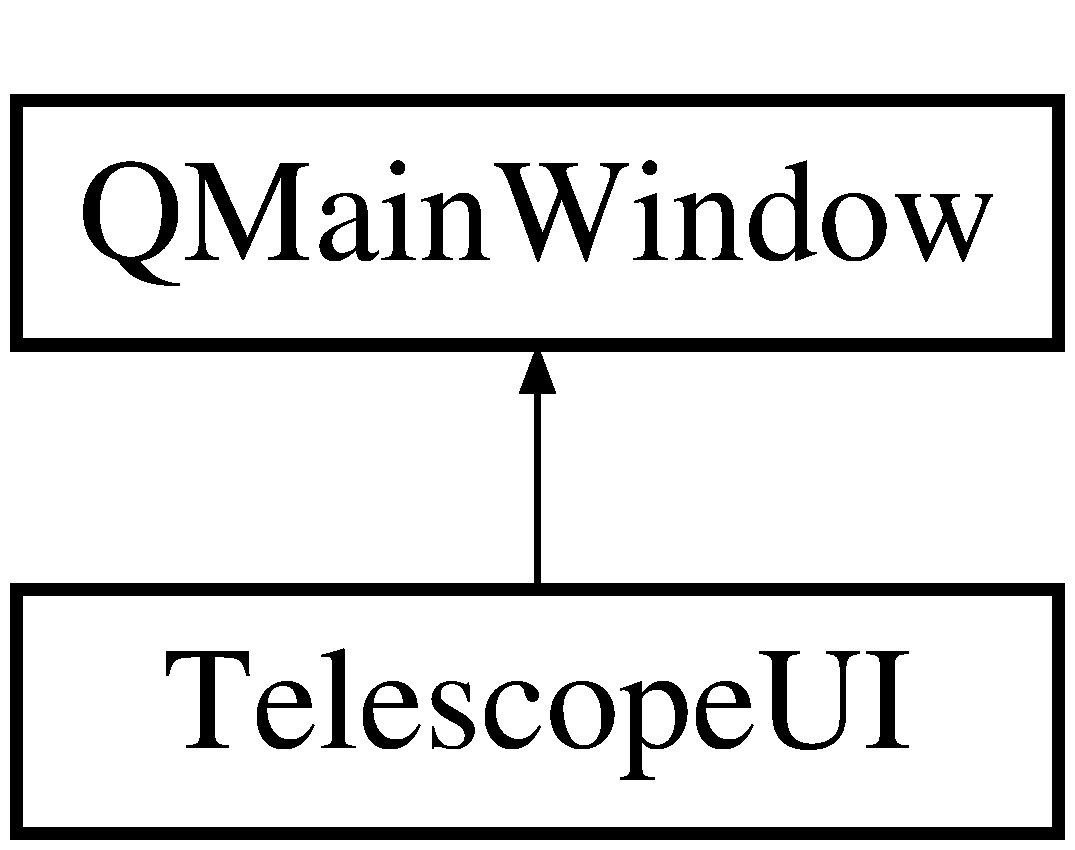
\includegraphics[height=2.000000cm]{classTelescopeUI}
\end{center}
\end{figure}
\subsection*{Public Member Functions}
\begin{DoxyCompactItemize}
\item 
\mbox{\hyperlink{classTelescopeUI_a15dc7e30e1387dc23213bec7ca74012c}{Telescope\+UI}} (\mbox{\hyperlink{classBackend}{Backend}} $\ast$const, Q\+Widget $\ast$parent=Q\+\_\+\+N\+U\+L\+L\+P\+TR)
\begin{DoxyCompactList}\small\item\em Main constructor for \mbox{\hyperlink{classRaspberryPiUtility}{Raspberry\+Pi\+Utility}} class. \end{DoxyCompactList}\item 
double \mbox{\hyperlink{classTelescopeUI_a617d9d50d6e4a50f58bf65658b2191b8}{get\+\_\+yaw\+\_\+input}} () const
\begin{DoxyCompactList}\small\item\em Getter method for yaw input from UI. \end{DoxyCompactList}\item 
double \mbox{\hyperlink{classTelescopeUI_a874796893c7941992ed16760d62409c5}{get\+\_\+pitch\+\_\+input}} () const
\begin{DoxyCompactList}\small\item\em Getter method for pitch input from UI. \end{DoxyCompactList}\item 
double \mbox{\hyperlink{classTelescopeUI_a1d2675c14ee541617257b68cef48b857}{get\+\_\+pitch\+\_\+vel\+\_\+input}} () const
\begin{DoxyCompactList}\small\item\em Getter method for pitch velocity input from UI. \end{DoxyCompactList}\item 
double \mbox{\hyperlink{classTelescopeUI_a5e3914156cf53cb53851285186d3fbfc}{get\+\_\+yaw\+\_\+vel\+\_\+input}} () const
\begin{DoxyCompactList}\small\item\em Getter method for yaw velocity input from UI. \end{DoxyCompactList}\item 
std\+::string \mbox{\hyperlink{classTelescopeUI_a6253863c7f48f2f403b44e1811f6dd2b}{get\+\_\+star\+\_\+input}} () const
\begin{DoxyCompactList}\small\item\em Getter method for star name input from UI. \end{DoxyCompactList}\item 
std\+::string \mbox{\hyperlink{classTelescopeUI_a821001a5b68adc425ca4b5abf40c1d20}{get\+\_\+planet\+\_\+input}} () const
\begin{DoxyCompactList}\small\item\em Getter method for planet name input from UI. \end{DoxyCompactList}\item 
void \mbox{\hyperlink{classTelescopeUI_ac228bd23c7e759df5aa81206872214b5}{set\+\_\+yaw\+\_\+output}} (double v)
\begin{DoxyCompactList}\small\item\em Setter method for displaying yaw on UI \textquotesingle{}L\+CD display\textquotesingle{}. \end{DoxyCompactList}\item 
void \mbox{\hyperlink{classTelescopeUI_a4388ce748e1ad31dbb5d9d4df38c750b}{set\+\_\+pitch\+\_\+output}} (double v)
\begin{DoxyCompactList}\small\item\em Setter method for displaying pitch on UI \textquotesingle{}L\+CD display\textquotesingle{}. \end{DoxyCompactList}\item 
void \mbox{\hyperlink{classTelescopeUI_a3d767f297da01b6cb685578ed2479e25}{set\+\_\+pitch\+\_\+vel\+\_\+output}} (double v)
\begin{DoxyCompactList}\small\item\em Setter method for displaying pitch velocity on UI \textquotesingle{}L\+CD display\textquotesingle{}. \end{DoxyCompactList}\item 
void \mbox{\hyperlink{classTelescopeUI_aa606620872e1d9402b74c26664d12c3d}{set\+\_\+yaw\+\_\+vel\+\_\+output}} (double v)
\begin{DoxyCompactList}\small\item\em Setter method for displaying yaw velocity on UI \textquotesingle{}L\+CD display\textquotesingle{}. \end{DoxyCompactList}\item 
void \mbox{\hyperlink{classTelescopeUI_a3761db8f2002e52be63df7cab0bf6167}{append\+\_\+console}} (std\+::string line)
\begin{DoxyCompactList}\small\item\em Setter method for writing lines to internal UI console. \end{DoxyCompactList}\item 
void \mbox{\hyperlink{classTelescopeUI_aa4bddc57881d00dd145312c84467ac1d}{set\+\_\+time\+\_\+dis}} (std\+::string line)
\begin{DoxyCompactList}\small\item\em Setter method for time display. \end{DoxyCompactList}\item 
void \mbox{\hyperlink{classTelescopeUI_aaf63d404f0d3ca0aaa53d8319255ac32}{set\+\_\+lat\+\_\+dis}} (std\+::string line)
\begin{DoxyCompactList}\small\item\em Setter method for latitude display. \end{DoxyCompactList}\item 
void \mbox{\hyperlink{classTelescopeUI_a17bbaf5bd8d520f6db7ccff5d20e2b15}{set\+\_\+long\+\_\+dis}} (std\+::string line)
\begin{DoxyCompactList}\small\item\em Setter method for longitude display. \end{DoxyCompactList}\item 
void \mbox{\hyperlink{classTelescopeUI_ae2e354a53baf9ad21263e0123b47785a}{set\+\_\+name\+\_\+dis}} (std\+::string line)
\begin{DoxyCompactList}\small\item\em Setter method for star/planet name display. \end{DoxyCompactList}\item 
void \mbox{\hyperlink{classTelescopeUI_a9af61f40fd39d3c22ecd349a038ef2b5}{set\+\_\+rasc\+\_\+dis}} (std\+::string line)
\begin{DoxyCompactList}\small\item\em Setter method for right ascension display. \end{DoxyCompactList}\item 
void \mbox{\hyperlink{classTelescopeUI_a783632af5cec9a781f0228204b7d4126}{set\+\_\+dec\+\_\+dis}} (std\+::string line)
\begin{DoxyCompactList}\small\item\em Setter method for declination display. \end{DoxyCompactList}\end{DoxyCompactItemize}
\subsection*{Private Attributes}
\begin{DoxyCompactItemize}
\item 
\mbox{\Hypertarget{classTelescopeUI_ac00c9f2b983cbb014fb21e4a9f5e76c9}\label{classTelescopeUI_ac00c9f2b983cbb014fb21e4a9f5e76c9}} 
Ui\+::\+Raspberry\+Pi\+Utility\+Class \mbox{\hyperlink{classTelescopeUI_ac00c9f2b983cbb014fb21e4a9f5e76c9}{ui}}
\begin{DoxyCompactList}\small\item\em References Qt UI elements from the template. \end{DoxyCompactList}\end{DoxyCompactItemize}


\subsection{Detailed Description}
$<$ Qt template UI generated using Qt Creator 

\subsection{Constructor \& Destructor Documentation}
\mbox{\Hypertarget{classTelescopeUI_a15dc7e30e1387dc23213bec7ca74012c}\label{classTelescopeUI_a15dc7e30e1387dc23213bec7ca74012c}} 
\index{Telescope\+UI@{Telescope\+UI}!Telescope\+UI@{Telescope\+UI}}
\index{Telescope\+UI@{Telescope\+UI}!Telescope\+UI@{Telescope\+UI}}
\subsubsection{\texorpdfstring{Telescope\+U\+I()}{TelescopeUI()}}
{\footnotesize\ttfamily Telescope\+U\+I\+::\+Telescope\+UI (\begin{DoxyParamCaption}\item[{\mbox{\hyperlink{classBackend}{Backend}} $\ast$ const}]{b,  }\item[{Q\+Widget $\ast$}]{parent = {\ttfamily Q\+\_\+NULLPTR} }\end{DoxyParamCaption})}



Main constructor for \mbox{\hyperlink{classRaspberryPiUtility}{Raspberry\+Pi\+Utility}} class. 

Implementation of main constructor for \mbox{\hyperlink{classRaspberryPiUtility}{Raspberry\+Pi\+Utility}}. Creates an instance of the Qt UI template, forming the UI for Telescope\+Control.


\begin{DoxyParams}{Parameters}
{\em Constant} & backend wrapper as pointer \\
\hline
{\em parent} & pointer of type Q\+Widget\\
\hline
{\em b} & pointer of type \mbox{\hyperlink{classBackend}{Backend}} \\
\hline
{\em parent} & pointer of type Q\+Widget \\
\hline
\end{DoxyParams}
$<$ Creates UI elements 

\subsection{Member Function Documentation}
\mbox{\Hypertarget{classTelescopeUI_a3761db8f2002e52be63df7cab0bf6167}\label{classTelescopeUI_a3761db8f2002e52be63df7cab0bf6167}} 
\index{Telescope\+UI@{Telescope\+UI}!append\+\_\+console@{append\+\_\+console}}
\index{append\+\_\+console@{append\+\_\+console}!Telescope\+UI@{Telescope\+UI}}
\subsubsection{\texorpdfstring{append\+\_\+console()}{append\_console()}}
{\footnotesize\ttfamily void Telescope\+U\+I\+::append\+\_\+console (\begin{DoxyParamCaption}\item[{std\+::string}]{line }\end{DoxyParamCaption})}



Setter method for writing lines to internal UI console. 


\begin{DoxyParams}{Parameters}
{\em String} & that contains the line to be displayed on the console \\
\hline
\end{DoxyParams}
\mbox{\Hypertarget{classTelescopeUI_a874796893c7941992ed16760d62409c5}\label{classTelescopeUI_a874796893c7941992ed16760d62409c5}} 
\index{Telescope\+UI@{Telescope\+UI}!get\+\_\+pitch\+\_\+input@{get\+\_\+pitch\+\_\+input}}
\index{get\+\_\+pitch\+\_\+input@{get\+\_\+pitch\+\_\+input}!Telescope\+UI@{Telescope\+UI}}
\subsubsection{\texorpdfstring{get\+\_\+pitch\+\_\+input()}{get\_pitch\_input()}}
{\footnotesize\ttfamily double Telescope\+U\+I\+::get\+\_\+pitch\+\_\+input (\begin{DoxyParamCaption}{ }\end{DoxyParamCaption}) const}



Getter method for pitch input from UI. 

\begin{DoxyReturn}{Returns}
double value for pitch 
\end{DoxyReturn}
\mbox{\Hypertarget{classTelescopeUI_a1d2675c14ee541617257b68cef48b857}\label{classTelescopeUI_a1d2675c14ee541617257b68cef48b857}} 
\index{Telescope\+UI@{Telescope\+UI}!get\+\_\+pitch\+\_\+vel\+\_\+input@{get\+\_\+pitch\+\_\+vel\+\_\+input}}
\index{get\+\_\+pitch\+\_\+vel\+\_\+input@{get\+\_\+pitch\+\_\+vel\+\_\+input}!Telescope\+UI@{Telescope\+UI}}
\subsubsection{\texorpdfstring{get\+\_\+pitch\+\_\+vel\+\_\+input()}{get\_pitch\_vel\_input()}}
{\footnotesize\ttfamily double Telescope\+U\+I\+::get\+\_\+pitch\+\_\+vel\+\_\+input (\begin{DoxyParamCaption}{ }\end{DoxyParamCaption}) const}



Getter method for pitch velocity input from UI. 

\begin{DoxyReturn}{Returns}
double value for velocity 
\end{DoxyReturn}
\mbox{\Hypertarget{classTelescopeUI_a821001a5b68adc425ca4b5abf40c1d20}\label{classTelescopeUI_a821001a5b68adc425ca4b5abf40c1d20}} 
\index{Telescope\+UI@{Telescope\+UI}!get\+\_\+planet\+\_\+input@{get\+\_\+planet\+\_\+input}}
\index{get\+\_\+planet\+\_\+input@{get\+\_\+planet\+\_\+input}!Telescope\+UI@{Telescope\+UI}}
\subsubsection{\texorpdfstring{get\+\_\+planet\+\_\+input()}{get\_planet\_input()}}
{\footnotesize\ttfamily std\+::string Telescope\+U\+I\+::get\+\_\+planet\+\_\+input (\begin{DoxyParamCaption}{ }\end{DoxyParamCaption}) const}



Getter method for planet name input from UI. 

\begin{DoxyReturn}{Returns}
string with planet name 
\end{DoxyReturn}
\mbox{\Hypertarget{classTelescopeUI_a6253863c7f48f2f403b44e1811f6dd2b}\label{classTelescopeUI_a6253863c7f48f2f403b44e1811f6dd2b}} 
\index{Telescope\+UI@{Telescope\+UI}!get\+\_\+star\+\_\+input@{get\+\_\+star\+\_\+input}}
\index{get\+\_\+star\+\_\+input@{get\+\_\+star\+\_\+input}!Telescope\+UI@{Telescope\+UI}}
\subsubsection{\texorpdfstring{get\+\_\+star\+\_\+input()}{get\_star\_input()}}
{\footnotesize\ttfamily std\+::string Telescope\+U\+I\+::get\+\_\+star\+\_\+input (\begin{DoxyParamCaption}{ }\end{DoxyParamCaption}) const}



Getter method for star name input from UI. 

\begin{DoxyReturn}{Returns}
string with star name 
\end{DoxyReturn}
\mbox{\Hypertarget{classTelescopeUI_a617d9d50d6e4a50f58bf65658b2191b8}\label{classTelescopeUI_a617d9d50d6e4a50f58bf65658b2191b8}} 
\index{Telescope\+UI@{Telescope\+UI}!get\+\_\+yaw\+\_\+input@{get\+\_\+yaw\+\_\+input}}
\index{get\+\_\+yaw\+\_\+input@{get\+\_\+yaw\+\_\+input}!Telescope\+UI@{Telescope\+UI}}
\subsubsection{\texorpdfstring{get\+\_\+yaw\+\_\+input()}{get\_yaw\_input()}}
{\footnotesize\ttfamily double Telescope\+U\+I\+::get\+\_\+yaw\+\_\+input (\begin{DoxyParamCaption}{ }\end{DoxyParamCaption}) const}



Getter method for yaw input from UI. 

\begin{DoxyReturn}{Returns}
double value for yaw 
\end{DoxyReturn}
\mbox{\Hypertarget{classTelescopeUI_a5e3914156cf53cb53851285186d3fbfc}\label{classTelescopeUI_a5e3914156cf53cb53851285186d3fbfc}} 
\index{Telescope\+UI@{Telescope\+UI}!get\+\_\+yaw\+\_\+vel\+\_\+input@{get\+\_\+yaw\+\_\+vel\+\_\+input}}
\index{get\+\_\+yaw\+\_\+vel\+\_\+input@{get\+\_\+yaw\+\_\+vel\+\_\+input}!Telescope\+UI@{Telescope\+UI}}
\subsubsection{\texorpdfstring{get\+\_\+yaw\+\_\+vel\+\_\+input()}{get\_yaw\_vel\_input()}}
{\footnotesize\ttfamily double Telescope\+U\+I\+::get\+\_\+yaw\+\_\+vel\+\_\+input (\begin{DoxyParamCaption}{ }\end{DoxyParamCaption}) const}



Getter method for yaw velocity input from UI. 

\begin{DoxyReturn}{Returns}
double value for velocity 
\end{DoxyReturn}
\mbox{\Hypertarget{classTelescopeUI_a783632af5cec9a781f0228204b7d4126}\label{classTelescopeUI_a783632af5cec9a781f0228204b7d4126}} 
\index{Telescope\+UI@{Telescope\+UI}!set\+\_\+dec\+\_\+dis@{set\+\_\+dec\+\_\+dis}}
\index{set\+\_\+dec\+\_\+dis@{set\+\_\+dec\+\_\+dis}!Telescope\+UI@{Telescope\+UI}}
\subsubsection{\texorpdfstring{set\+\_\+dec\+\_\+dis()}{set\_dec\_dis()}}
{\footnotesize\ttfamily void Telescope\+U\+I\+::set\+\_\+dec\+\_\+dis (\begin{DoxyParamCaption}\item[{std\+::string}]{line }\end{DoxyParamCaption})}



Setter method for declination display. 


\begin{DoxyParams}{Parameters}
{\em line} & contains declination as string \\
\hline
\end{DoxyParams}
\mbox{\Hypertarget{classTelescopeUI_aaf63d404f0d3ca0aaa53d8319255ac32}\label{classTelescopeUI_aaf63d404f0d3ca0aaa53d8319255ac32}} 
\index{Telescope\+UI@{Telescope\+UI}!set\+\_\+lat\+\_\+dis@{set\+\_\+lat\+\_\+dis}}
\index{set\+\_\+lat\+\_\+dis@{set\+\_\+lat\+\_\+dis}!Telescope\+UI@{Telescope\+UI}}
\subsubsection{\texorpdfstring{set\+\_\+lat\+\_\+dis()}{set\_lat\_dis()}}
{\footnotesize\ttfamily void Telescope\+U\+I\+::set\+\_\+lat\+\_\+dis (\begin{DoxyParamCaption}\item[{std\+::string}]{line }\end{DoxyParamCaption})}



Setter method for latitude display. 


\begin{DoxyParams}{Parameters}
{\em line} & contains latitude as string \\
\hline
\end{DoxyParams}
\mbox{\Hypertarget{classTelescopeUI_a17bbaf5bd8d520f6db7ccff5d20e2b15}\label{classTelescopeUI_a17bbaf5bd8d520f6db7ccff5d20e2b15}} 
\index{Telescope\+UI@{Telescope\+UI}!set\+\_\+long\+\_\+dis@{set\+\_\+long\+\_\+dis}}
\index{set\+\_\+long\+\_\+dis@{set\+\_\+long\+\_\+dis}!Telescope\+UI@{Telescope\+UI}}
\subsubsection{\texorpdfstring{set\+\_\+long\+\_\+dis()}{set\_long\_dis()}}
{\footnotesize\ttfamily void Telescope\+U\+I\+::set\+\_\+long\+\_\+dis (\begin{DoxyParamCaption}\item[{std\+::string}]{line }\end{DoxyParamCaption})}



Setter method for longitude display. 


\begin{DoxyParams}{Parameters}
{\em line} & contains longitude as string \\
\hline
\end{DoxyParams}
\mbox{\Hypertarget{classTelescopeUI_ae2e354a53baf9ad21263e0123b47785a}\label{classTelescopeUI_ae2e354a53baf9ad21263e0123b47785a}} 
\index{Telescope\+UI@{Telescope\+UI}!set\+\_\+name\+\_\+dis@{set\+\_\+name\+\_\+dis}}
\index{set\+\_\+name\+\_\+dis@{set\+\_\+name\+\_\+dis}!Telescope\+UI@{Telescope\+UI}}
\subsubsection{\texorpdfstring{set\+\_\+name\+\_\+dis()}{set\_name\_dis()}}
{\footnotesize\ttfamily void Telescope\+U\+I\+::set\+\_\+name\+\_\+dis (\begin{DoxyParamCaption}\item[{std\+::string}]{line }\end{DoxyParamCaption})}



Setter method for star/planet name display. 


\begin{DoxyParams}{Parameters}
{\em line} & contains star/name as string \\
\hline
\end{DoxyParams}
\mbox{\Hypertarget{classTelescopeUI_a4388ce748e1ad31dbb5d9d4df38c750b}\label{classTelescopeUI_a4388ce748e1ad31dbb5d9d4df38c750b}} 
\index{Telescope\+UI@{Telescope\+UI}!set\+\_\+pitch\+\_\+output@{set\+\_\+pitch\+\_\+output}}
\index{set\+\_\+pitch\+\_\+output@{set\+\_\+pitch\+\_\+output}!Telescope\+UI@{Telescope\+UI}}
\subsubsection{\texorpdfstring{set\+\_\+pitch\+\_\+output()}{set\_pitch\_output()}}
{\footnotesize\ttfamily void Telescope\+U\+I\+::set\+\_\+pitch\+\_\+output (\begin{DoxyParamCaption}\item[{double}]{v }\end{DoxyParamCaption})}



Setter method for displaying pitch on UI \textquotesingle{}L\+CD display\textquotesingle{}. 


\begin{DoxyParams}{Parameters}
{\em v} & represents double value for pitch \\
\hline
\end{DoxyParams}
\mbox{\Hypertarget{classTelescopeUI_a3d767f297da01b6cb685578ed2479e25}\label{classTelescopeUI_a3d767f297da01b6cb685578ed2479e25}} 
\index{Telescope\+UI@{Telescope\+UI}!set\+\_\+pitch\+\_\+vel\+\_\+output@{set\+\_\+pitch\+\_\+vel\+\_\+output}}
\index{set\+\_\+pitch\+\_\+vel\+\_\+output@{set\+\_\+pitch\+\_\+vel\+\_\+output}!Telescope\+UI@{Telescope\+UI}}
\subsubsection{\texorpdfstring{set\+\_\+pitch\+\_\+vel\+\_\+output()}{set\_pitch\_vel\_output()}}
{\footnotesize\ttfamily void Telescope\+U\+I\+::set\+\_\+pitch\+\_\+vel\+\_\+output (\begin{DoxyParamCaption}\item[{double}]{v }\end{DoxyParamCaption})}



Setter method for displaying pitch velocity on UI \textquotesingle{}L\+CD display\textquotesingle{}. 


\begin{DoxyParams}{Parameters}
{\em v} & represents double value for velocity \\
\hline
\end{DoxyParams}
\mbox{\Hypertarget{classTelescopeUI_a9af61f40fd39d3c22ecd349a038ef2b5}\label{classTelescopeUI_a9af61f40fd39d3c22ecd349a038ef2b5}} 
\index{Telescope\+UI@{Telescope\+UI}!set\+\_\+rasc\+\_\+dis@{set\+\_\+rasc\+\_\+dis}}
\index{set\+\_\+rasc\+\_\+dis@{set\+\_\+rasc\+\_\+dis}!Telescope\+UI@{Telescope\+UI}}
\subsubsection{\texorpdfstring{set\+\_\+rasc\+\_\+dis()}{set\_rasc\_dis()}}
{\footnotesize\ttfamily void Telescope\+U\+I\+::set\+\_\+rasc\+\_\+dis (\begin{DoxyParamCaption}\item[{std\+::string}]{line }\end{DoxyParamCaption})}



Setter method for right ascension display. 


\begin{DoxyParams}{Parameters}
{\em line} & contains right ascension as string \\
\hline
\end{DoxyParams}
\mbox{\Hypertarget{classTelescopeUI_aa4bddc57881d00dd145312c84467ac1d}\label{classTelescopeUI_aa4bddc57881d00dd145312c84467ac1d}} 
\index{Telescope\+UI@{Telescope\+UI}!set\+\_\+time\+\_\+dis@{set\+\_\+time\+\_\+dis}}
\index{set\+\_\+time\+\_\+dis@{set\+\_\+time\+\_\+dis}!Telescope\+UI@{Telescope\+UI}}
\subsubsection{\texorpdfstring{set\+\_\+time\+\_\+dis()}{set\_time\_dis()}}
{\footnotesize\ttfamily void Telescope\+U\+I\+::set\+\_\+time\+\_\+dis (\begin{DoxyParamCaption}\item[{std\+::string}]{line }\end{DoxyParamCaption})}



Setter method for time display. 


\begin{DoxyParams}{Parameters}
{\em line} & contains time as string \\
\hline
\end{DoxyParams}
\mbox{\Hypertarget{classTelescopeUI_ac228bd23c7e759df5aa81206872214b5}\label{classTelescopeUI_ac228bd23c7e759df5aa81206872214b5}} 
\index{Telescope\+UI@{Telescope\+UI}!set\+\_\+yaw\+\_\+output@{set\+\_\+yaw\+\_\+output}}
\index{set\+\_\+yaw\+\_\+output@{set\+\_\+yaw\+\_\+output}!Telescope\+UI@{Telescope\+UI}}
\subsubsection{\texorpdfstring{set\+\_\+yaw\+\_\+output()}{set\_yaw\_output()}}
{\footnotesize\ttfamily void Telescope\+U\+I\+::set\+\_\+yaw\+\_\+output (\begin{DoxyParamCaption}\item[{double}]{v }\end{DoxyParamCaption})}



Setter method for displaying yaw on UI \textquotesingle{}L\+CD display\textquotesingle{}. 


\begin{DoxyParams}{Parameters}
{\em v} & represents double value for yaw \\
\hline
\end{DoxyParams}
\mbox{\Hypertarget{classTelescopeUI_aa606620872e1d9402b74c26664d12c3d}\label{classTelescopeUI_aa606620872e1d9402b74c26664d12c3d}} 
\index{Telescope\+UI@{Telescope\+UI}!set\+\_\+yaw\+\_\+vel\+\_\+output@{set\+\_\+yaw\+\_\+vel\+\_\+output}}
\index{set\+\_\+yaw\+\_\+vel\+\_\+output@{set\+\_\+yaw\+\_\+vel\+\_\+output}!Telescope\+UI@{Telescope\+UI}}
\subsubsection{\texorpdfstring{set\+\_\+yaw\+\_\+vel\+\_\+output()}{set\_yaw\_vel\_output()}}
{\footnotesize\ttfamily void Telescope\+U\+I\+::set\+\_\+yaw\+\_\+vel\+\_\+output (\begin{DoxyParamCaption}\item[{double}]{v }\end{DoxyParamCaption})}



Setter method for displaying yaw velocity on UI \textquotesingle{}L\+CD display\textquotesingle{}. 


\begin{DoxyParams}{Parameters}
{\em v} & represents double value for velocity \\
\hline
\end{DoxyParams}


The documentation for this class was generated from the following files\+:\begin{DoxyCompactItemize}
\item 
telescopeui.\+h\item 
telescopeui.\+cpp\end{DoxyCompactItemize}

\hypertarget{classtmc}{}\section{tmc Class Reference}
\label{classtmc}\index{tmc@{tmc}}


The documentation for this class was generated from the following file\+:\begin{DoxyCompactItemize}
\item 
translation.\+h\end{DoxyCompactItemize}

\hypertarget{classweb}{}\section{web Class Reference}
\label{classweb}\index{web@{web}}


The documentation for this class was generated from the following file\+:\begin{DoxyCompactItemize}
\item 
\mbox{\hyperlink{downloadpage_8h}{downloadpage.\+h}}\end{DoxyCompactItemize}

\chapter{File Documentation}
\hypertarget{Angle_8cpp}{}\section{Angle.\+cpp File Reference}
\label{Angle_8cpp}\index{Angle.\+cpp@{Angle.\+cpp}}


\mbox{\hyperlink{classAngle}{Angle}} class represents angular measurements and allows conversion between different units.  


{\ttfamily \#include \char`\"{}Angle.\+h\char`\"{}}\newline
{\ttfamily \#include $<$math.\+h$>$}\newline


\subsection{Detailed Description}
\mbox{\hyperlink{classAngle}{Angle}} class represents angular measurements and allows conversion between different units. 

Implements \mbox{\hyperlink{Angle_8h}{Angle.\+h}} header \begin{DoxyAuthor}{Authors}
Matt Abado, Christian Wrona 
\end{DoxyAuthor}
\begin{DoxyDate}{Date}
2018-\/11 
\end{DoxyDate}

\hypertarget{Angle_8h}{}\section{Angle.\+h File Reference}
\label{Angle_8h}\index{Angle.\+h@{Angle.\+h}}


\mbox{\hyperlink{classAngle}{Angle}} class represents angular measurements and allows conversion between different units.  


{\ttfamily \#include $<$string$>$}\newline
{\ttfamily \#include $<$map$>$}\newline
\subsection*{Classes}
\begin{DoxyCompactItemize}
\item 
class \mbox{\hyperlink{classAngle}{Angle}}
\end{DoxyCompactItemize}


\subsection{Detailed Description}
\mbox{\hyperlink{classAngle}{Angle}} class represents angular measurements and allows conversion between different units. 

\begin{DoxyAuthor}{Authors}
Matt Abado, Christian Wrona 
\end{DoxyAuthor}
\begin{DoxyDate}{Date}
2018-\/11 
\end{DoxyDate}

\hypertarget{celestialdb_8h}{}\section{celestialdb.\+h File Reference}
\label{celestialdb_8h}\index{celestialdb.\+h@{celestialdb.\+h}}


Implements Celestial Database.  


{\ttfamily \#include $<$iostream$>$}\newline
\subsection*{Classes}
\begin{DoxyCompactItemize}
\item 
class \mbox{\hyperlink{structCelestialDB}{Celestial\+DB}}
\end{DoxyCompactItemize}


\subsection{Detailed Description}
Implements Celestial Database. 

\begin{DoxyAuthor}{Authors}
Steve Silber 
\end{DoxyAuthor}
\begin{DoxyDate}{Date}
2018-\/11 
\end{DoxyDate}

\hypertarget{celestialin_8h}{}\section{celestialin.\+h File Reference}
\label{celestialin_8h}\index{celestialin.\+h@{celestialin.\+h}}


Bridge between celestialdb class and UI.  


{\ttfamily \#include \char`\"{}bridgein.\+h\char`\"{}}\newline
{\ttfamily \#include \char`\"{}telescopeui.\+h\char`\"{}}\newline
{\ttfamily \#include \char`\"{}control.\+h\char`\"{}}\newline
{\ttfamily \#include \char`\"{}celestialdb.\+h\char`\"{}}\newline
\subsection*{Classes}
\begin{DoxyCompactItemize}
\item 
class \mbox{\hyperlink{classCelestialIn}{Celestial\+In}}
\end{DoxyCompactItemize}


\subsection{Detailed Description}
Bridge between celestialdb class and UI. 

\begin{DoxyAuthor}{Authors}
Steve Silber, Alex Yan 
\end{DoxyAuthor}
\begin{DoxyDate}{Date}
2018-\/11 
\end{DoxyDate}

\hypertarget{control_8h}{}\section{control.\+h File Reference}
\label{control_8h}\index{control.\+h@{control.\+h}}


the A\+PI for the Telescope Motor Control there is no function to read the current coordinates as the design does not allow the motor control to be polled  


{\ttfamily \#include $<$utility$>$}\newline
{\ttfamily \#include $<$thread$>$}\newline
{\ttfamily \#include \char`\"{}motorcontrol.\+h\char`\"{}}\newline
\subsection*{Typedefs}
\begin{DoxyCompactItemize}
\item 
\mbox{\Hypertarget{control_8h_a01df60c309a1b5500cc9d7c732ff3912}\label{control_8h_a01df60c309a1b5500cc9d7c732ff3912}} 
typedef double {\bfseries Degree}
\item 
\mbox{\Hypertarget{control_8h_a2cd3f46402e6c41c2d013b9184cae4a6}\label{control_8h_a2cd3f46402e6c41c2d013b9184cae4a6}} 
typedef double {\bfseries Real\+Angle}
\end{DoxyCompactItemize}
\subsection*{Functions}
\begin{DoxyCompactItemize}
\item 
{\footnotesize template$<$typename T  = decltype(\+\_\+\+\_\+no\+\_\+fn), typename ... Args$>$ }\\bool \mbox{\hyperlink{control_8h_a2697c723984cc0200677b73f7ac16ff5}{tmc\+::to\+\_\+coords}} (Degree yaw, Degree pitch, T end\+\_\+fn=\+\_\+\+\_\+no\+\_\+fn, Args ...fn\+\_\+args)
\begin{DoxyCompactList}\small\item\em takes a pair of coordinates as a destination to move the telescope to returns the coordinates before initiating the move this function is N\+O\+N\+B\+L\+O\+C\+K\+I\+NG \end{DoxyCompactList}\item 
{\footnotesize template$<$typename T  = decltype(\+\_\+\+\_\+no\+\_\+fn), typename ... Args$>$ }\\bool \mbox{\hyperlink{control_8h_a41f34fdf6f02923fbdef84fd40bc19be}{tmc\+::set\+\_\+velocity}} (Degree yaw, Degree pitch, T end\+\_\+fn=\+\_\+\+\_\+no\+\_\+fn, Args ...fn\+\_\+args)
\begin{DoxyCompactList}\small\item\em takes a pair of velocity coordinates, which will persistently move the telescope until stop is called or end of freedom of motion is reached returns the coordinates before initiating the translation this function is N\+O\+N\+B\+L\+O\+C\+K\+I\+NG \end{DoxyCompactList}\item 
\mbox{\Hypertarget{control_8h_aaa1bc8395514b80a9fc58b7f122d94b6}\label{control_8h_aaa1bc8395514b80a9fc58b7f122d94b6}} 
std\+::pair$<$ Degree, Degree $>$ {\bfseries tmc\+::get\+\_\+coords} ()
\item 
{\footnotesize template$<$typename T  = decltype(\+\_\+\+\_\+no\+\_\+fn), typename ... Args$>$ }\\std\+::pair$<$ double, double $>$ \mbox{\hyperlink{control_8h_af21f73ad3fc6aaafe7d0e4e9127fe02d}{tmc\+::stop}} (T on\+\_\+stop)
\begin{DoxyCompactList}\small\item\em calls an all stop on the telescope movement, if the telescope isn\textquotesingle{}t moving, there is no effect \end{DoxyCompactList}\end{DoxyCompactItemize}
\subsection*{Variables}
\begin{DoxyCompactItemize}
\item 
\mbox{\Hypertarget{control_8h_a44f6d174372cad3b4035dc5ff8941d4a}\label{control_8h_a44f6d174372cad3b4035dc5ff8941d4a}} 
static void($\ast$ {\bfseries \+\_\+\+\_\+no\+\_\+fn} )() = \mbox{[}$\,$\mbox{]}() \{\}
\end{DoxyCompactItemize}


\subsection{Detailed Description}
the A\+PI for the Telescope Motor Control there is no function to read the current coordinates as the design does not allow the motor control to be polled 

\begin{DoxyAuthor}{Authors}
Steve Silber, Alex Yan 
\end{DoxyAuthor}
\begin{DoxyDate}{Date}
2018-\/11 
\end{DoxyDate}


\subsection{Function Documentation}
\mbox{\Hypertarget{control_8h_file_a41f34fdf6f02923fbdef84fd40bc19be}\label{control_8h_file_a41f34fdf6f02923fbdef84fd40bc19be}} 
\index{control.\+h@{control.\+h}!set\+\_\+velocity@{set\+\_\+velocity}}
\index{set\+\_\+velocity@{set\+\_\+velocity}!control.\+h@{control.\+h}}
\subsubsection{\texorpdfstring{set\+\_\+velocity()}{set\_velocity()}}
{\footnotesize\ttfamily template$<$typename T  = decltype(\+\_\+\+\_\+no\+\_\+fn), typename ... Args$>$ \\
bool tmc\+::set\+\_\+velocity (\begin{DoxyParamCaption}\item[{Degree}]{yaw,  }\item[{Degree}]{pitch,  }\item[{T}]{end\+\_\+fn = {\ttfamily \+\_\+\+\_\+no\+\_\+fn},  }\item[{Args ...}]{fn\+\_\+args }\end{DoxyParamCaption})}



takes a pair of velocity coordinates, which will persistently move the telescope until stop is called or end of freedom of motion is reached returns the coordinates before initiating the translation this function is N\+O\+N\+B\+L\+O\+C\+K\+I\+NG 


\begin{DoxyParams}{Parameters}
{\em yaw} & The yaw value to act as speed in horizontal direction \\
\hline
{\em pitch} & The pitch value to act as speed in vertical direction \\
\hline
{\em end\+\_\+fn} & The function that\textquotesingle{}s called when the motor activity finishes \\
\hline
{\em fn\+\_\+args} & Arguments passed to the end\+\_\+fn function \\
\hline
\end{DoxyParams}
\mbox{\Hypertarget{control_8h_file_af21f73ad3fc6aaafe7d0e4e9127fe02d}\label{control_8h_file_af21f73ad3fc6aaafe7d0e4e9127fe02d}} 
\index{control.\+h@{control.\+h}!stop@{stop}}
\index{stop@{stop}!control.\+h@{control.\+h}}
\subsubsection{\texorpdfstring{stop()}{stop()}}
{\footnotesize\ttfamily template$<$typename T  = decltype(\+\_\+\+\_\+no\+\_\+fn), typename ... Args$>$ \\
std\+::pair$<$double, double$>$ tmc\+::stop (\begin{DoxyParamCaption}\item[{T}]{on\+\_\+stop }\end{DoxyParamCaption})}



calls an all stop on the telescope movement, if the telescope isn\textquotesingle{}t moving, there is no effect 

\begin{DoxyReturn}{Returns}
the coordinates after stopping returning the coordinates means that a stop command could be B\+L\+O\+C\+K\+I\+NG 
\end{DoxyReturn}
\mbox{\Hypertarget{control_8h_file_a2697c723984cc0200677b73f7ac16ff5}\label{control_8h_file_a2697c723984cc0200677b73f7ac16ff5}} 
\index{control.\+h@{control.\+h}!to\+\_\+coords@{to\+\_\+coords}}
\index{to\+\_\+coords@{to\+\_\+coords}!control.\+h@{control.\+h}}
\subsubsection{\texorpdfstring{to\+\_\+coords()}{to\_coords()}}
{\footnotesize\ttfamily template$<$typename T  = decltype(\+\_\+\+\_\+no\+\_\+fn), typename ... Args$>$ \\
bool tmc\+::to\+\_\+coords (\begin{DoxyParamCaption}\item[{Degree}]{yaw,  }\item[{Degree}]{pitch,  }\item[{T}]{end\+\_\+fn = {\ttfamily \+\_\+\+\_\+no\+\_\+fn},  }\item[{Args ...}]{fn\+\_\+args }\end{DoxyParamCaption})}



takes a pair of coordinates as a destination to move the telescope to returns the coordinates before initiating the move this function is N\+O\+N\+B\+L\+O\+C\+K\+I\+NG 


\begin{DoxyParams}{Parameters}
{\em yaw} & The yaw value to act as new position in horizontal direction \\
\hline
{\em pitch} & The pitch value to act as new position in vertical direction \\
\hline
{\em end\+\_\+fn} & The function that\textquotesingle{}s called when the motor activity finishes \\
\hline
{\em fn\+\_\+args} & Arguments passed to the end\+\_\+fn function \\
\hline
\end{DoxyParams}

\hypertarget{coordencoder_8h}{}\section{coordencoder.\+h File Reference}
\label{coordencoder_8h}\index{coordencoder.\+h@{coordencoder.\+h}}


Methods for converting coordinates into integers and bytes.  


{\ttfamily \#include $<$utility$>$}\newline
{\ttfamily \#include $<$iostream$>$}\newline
\subsection*{Macros}
\begin{DoxyCompactItemize}
\item 
\mbox{\Hypertarget{coordencoder_8h_aae57f17e11e61cf0519e2004414f5629}\label{coordencoder_8h_aae57f17e11e61cf0519e2004414f5629}} 
\#define {\bfseries S\+TR}(X)~\#X
\item 
\mbox{\Hypertarget{coordencoder_8h_a6c763b45c0045a25fe47cca85da2b7cf}\label{coordencoder_8h_a6c763b45c0045a25fe47cca85da2b7cf}} 
\#define {\bfseries M\+S\+G\+\_\+\+Y\+A\+W\+\_\+\+P\+OS}~16
\item 
\mbox{\Hypertarget{coordencoder_8h_a02edaed0940adc80b0351dc88e3d46ba}\label{coordencoder_8h_a02edaed0940adc80b0351dc88e3d46ba}} 
\#define {\bfseries M\+S\+G\+\_\+\+P\+I\+T\+C\+H\+\_\+\+P\+OS}~16
\item 
\mbox{\Hypertarget{coordencoder_8h_a5e694ff7e65ff3bc826720a88ba425f1}\label{coordencoder_8h_a5e694ff7e65ff3bc826720a88ba425f1}} 
\#define {\bfseries B\+I\+T\+\_\+\+L\+E\+N\+G\+TH}~(M\+S\+G\+\_\+\+Y\+A\+W\+\_\+\+P\+OS + M\+S\+G\+\_\+\+P\+I\+T\+C\+H\+\_\+\+P\+OS)
\item 
\mbox{\Hypertarget{coordencoder_8h_aa204ec58d846f2354e6bd239460db89f}\label{coordencoder_8h_aa204ec58d846f2354e6bd239460db89f}} 
\#define {\bfseries M\+S\+G\+\_\+\+L\+E\+N\+G\+TH}~(B\+I\+T\+\_\+\+L\+E\+N\+G\+TH $>$$>$ 3)
\item 
\mbox{\Hypertarget{coordencoder_8h_af8dd24004011a014ca1cd76e3946e933}\label{coordencoder_8h_af8dd24004011a014ca1cd76e3946e933}} 
\#define {\bfseries M\+S\+G\+\_\+\+F\+O\+R\+M\+AT}~(\char`\"{}\%\char`\"{} S\+TR(M\+S\+G\+\_\+\+Y\+A\+W\+\_\+\+P\+OS) \char`\"{}s\%\char`\"{} S\+TR(M\+S\+G\+\_\+\+P\+I\+T\+C\+H\+\_\+\+P\+OS) \char`\"{}s\char`\"{})
\item 
\mbox{\Hypertarget{coordencoder_8h_a2cacce89acb2845005978bb861cadf10}\label{coordencoder_8h_a2cacce89acb2845005978bb861cadf10}} 
\#define {\bfseries N\+O\+R\+M\+A\+L\+I\+Z\+A\+T\+I\+O\+N\+\_\+\+F\+A\+C\+T\+OR}~100.\+0
\end{DoxyCompactItemize}
\subsection*{Functions}
\begin{DoxyCompactItemize}
\item 
\mbox{\Hypertarget{coordencoder_8h_a2a6d400796615f27e6f2194a0d5b0dbf}\label{coordencoder_8h_a2a6d400796615f27e6f2194a0d5b0dbf}} 
void {\bfseries ce\+::coords\+\_\+to\+\_\+char} (double, double, char $\ast$)
\item 
\mbox{\Hypertarget{coordencoder_8h_a176c06a7673a9a38414eb0c6ce3daea6}\label{coordencoder_8h_a176c06a7673a9a38414eb0c6ce3daea6}} 
unsigned int {\bfseries ce\+::coords\+\_\+to\+\_\+int} (double, double)
\item 
\mbox{\Hypertarget{coordencoder_8h_a382ea64c237ac28db9e54fe6434c0817}\label{coordencoder_8h_a382ea64c237ac28db9e54fe6434c0817}} 
unsigned int {\bfseries ce\+::char\+\_\+to\+\_\+int} (char\mbox{[}M\+S\+G\+\_\+\+L\+E\+N\+G\+TH\mbox{]})
\item 
\mbox{\Hypertarget{coordencoder_8h_a5e204428474524b9308775d3d484c911}\label{coordencoder_8h_a5e204428474524b9308775d3d484c911}} 
std\+::pair$<$ double, double $>$ {\bfseries ce\+::bytes\+\_\+to\+\_\+coords} (char\mbox{[}M\+S\+G\+\_\+\+L\+E\+N\+G\+TH\mbox{]})
\item 
\mbox{\Hypertarget{coordencoder_8h_a082913882615ec86a18ca9cdce6cfa6a}\label{coordencoder_8h_a082913882615ec86a18ca9cdce6cfa6a}} 
std\+::pair$<$ double, double $>$ {\bfseries ce\+::bytes\+\_\+to\+\_\+coords} (unsigned int)
\item 
\mbox{\Hypertarget{coordencoder_8h_a108ae678702eb6bf87b495101bf5fb7c}\label{coordencoder_8h_a108ae678702eb6bf87b495101bf5fb7c}} 
void {\bfseries ce\+::print\+\_\+as\+\_\+bits} (unsigned int data, char $\ast$out)
\item 
\mbox{\Hypertarget{coordencoder_8h_aa8a7193c84fc53afb1dd6ee6ae6acd04}\label{coordencoder_8h_aa8a7193c84fc53afb1dd6ee6ae6acd04}} 
void {\bfseries ce\+::print\+\_\+as\+\_\+bits} (char $\ast$data, char $\ast$out)
\end{DoxyCompactItemize}


\subsection{Detailed Description}
Methods for converting coordinates into integers and bytes. 

\begin{DoxyAuthor}{Authors}
Steve Silber 
\end{DoxyAuthor}
\begin{DoxyDate}{Date}
2018-\/11 
\end{DoxyDate}

\hypertarget{coordinates_8h}{}\section{coordinates.\+h File Reference}
\label{coordinates_8h}\index{coordinates.\+h@{coordinates.\+h}}


Structures for equatorial coordinates.  


\subsection*{Classes}
\begin{DoxyCompactItemize}
\item 
class \mbox{\hyperlink{structrightasc}{rightasc}}
\item 
struct \mbox{\hyperlink{structdeclination}{declination}}
\end{DoxyCompactItemize}
\subsection*{Macros}
\begin{DoxyCompactItemize}
\item 
\mbox{\Hypertarget{coordinates_8h_aef663a328efd775a0421984fc2121aca}\label{coordinates_8h_aef663a328efd775a0421984fc2121aca}} 
\#define {\bfseries R\+I\+G\+H\+T\+\_\+\+A\+S\+C\+\_\+\+F\+MT}~\char`\"{}\%dh\%dm\%lfs\char`\"{}
\item 
\mbox{\Hypertarget{coordinates_8h_afd92d5956bd5a50bfef18b27c303c139}\label{coordinates_8h_afd92d5956bd5a50bfef18b27c303c139}} 
\#define {\bfseries D\+E\+C\+L\+I\+N\+A\+T\+I\+O\+N\+\_\+\+F\+MT}~\char`\"{}\%d$\ast$\%d\textquotesingle{}\%lf\char`\"{}
\end{DoxyCompactItemize}


\subsection{Detailed Description}
Structures for equatorial coordinates. 

\begin{DoxyAuthor}{Authors}
Steve Silber 
\end{DoxyAuthor}
\begin{DoxyDate}{Date}
2018-\/11 
\end{DoxyDate}

\hypertarget{downloadpage_8h}{}\section{downloadpage.\+h File Reference}
\label{downloadpage_8h}\index{downloadpage.\+h@{downloadpage.\+h}}


Implements retrieval of webpage data.  


{\ttfamily \#include $<$string$>$}\newline
{\ttfamily \#include $<$sys/socket.\+h$>$}\newline
{\ttfamily \#include $<$sys/un.\+h$>$}\newline
{\ttfamily \#include $<$Q\+Object$>$}\newline
{\ttfamily \#include $<$Q\+Byte\+Array$>$}\newline
{\ttfamily \#include $<$Q\+Network\+Access\+Manager$>$}\newline
{\ttfamily \#include $<$Q\+Network\+Request$>$}\newline
{\ttfamily \#include $<$Q\+Network\+Reply$>$}\newline
\subsection*{Macros}
\begin{DoxyCompactItemize}
\item 
\mbox{\Hypertarget{downloadpage_8h_a0b08432e3d84621c28ff812b51075e60}\label{downloadpage_8h_a0b08432e3d84621c28ff812b51075e60}} 
\#define {\bfseries H\+T\+T\+P\+\_\+\+B\+U\+F\+F\+E\+R\+\_\+\+S\+I\+ZE}~1 $<$$<$ 10
\item 
\mbox{\Hypertarget{downloadpage_8h_a38a2e2d91d49b07fa63cfc74eaff064a}\label{downloadpage_8h_a38a2e2d91d49b07fa63cfc74eaff064a}} 
\#define {\bfseries H\+T\+T\+P\+\_\+\+B\+U\+F\+F\+E\+R\+\_\+\+C\+O\+N\+T\+E\+NT}~1 $<$$<$ 16
\end{DoxyCompactItemize}
\subsection*{Functions}
\begin{DoxyCompactItemize}
\item 
bool \mbox{\hyperlink{downloadpage_8h_adac987ba32cf72179ea124859b819d63}{web\+::get\+\_\+page}} (char $\ast$contents, char $\ast$hostname, char $\ast$url)
\begin{DoxyCompactList}\small\item\em given the url of a webpage, it will download the plaintext http contents using either linux or windows utilities (based on the compilation system), since this waits for http reply, this function is blocking. \end{DoxyCompactList}\item 
bool \mbox{\hyperlink{downloadpage_8h_a71852ed4b99b72ac223924d4e43a39b9}{web\+::get\+\_\+page\+\_\+qt}} (char $\ast$contents, char $\ast$url)
\begin{DoxyCompactList}\small\item\em Given the url of a webpage, it will download the plaintext http contents using either linux or windows utilities (based on the compilation system), since this waits for http reply, this function is blocking. \end{DoxyCompactList}\end{DoxyCompactItemize}


\subsection{Detailed Description}
Implements retrieval of webpage data. 

\begin{DoxyAuthor}{Authors}
Steve Silber 
\end{DoxyAuthor}
\begin{DoxyDate}{Date}
2018-\/11 
\end{DoxyDate}


\subsection{Function Documentation}
\mbox{\Hypertarget{downloadpage_8h_file_adac987ba32cf72179ea124859b819d63}\label{downloadpage_8h_file_adac987ba32cf72179ea124859b819d63}} 
\index{downloadpage.\+h@{downloadpage.\+h}!get\+\_\+page@{get\+\_\+page}}
\index{get\+\_\+page@{get\+\_\+page}!downloadpage.\+h@{downloadpage.\+h}}
\subsubsection{\texorpdfstring{get\+\_\+page()}{get\_page()}}
{\footnotesize\ttfamily bool web\+::get\+\_\+page (\begin{DoxyParamCaption}\item[{char $\ast$}]{contents,  }\item[{char $\ast$}]{hostname,  }\item[{char $\ast$}]{url }\end{DoxyParamCaption})}



given the url of a webpage, it will download the plaintext http contents using either linux or windows utilities (based on the compilation system), since this waits for http reply, this function is blocking. 


\begin{DoxyParams}{Parameters}
{\em contents} & A string into which to download the webpage \\
\hline
{\em url} & The web location address of the webpage \\
\hline
\end{DoxyParams}
\mbox{\Hypertarget{downloadpage_8h_file_a71852ed4b99b72ac223924d4e43a39b9}\label{downloadpage_8h_file_a71852ed4b99b72ac223924d4e43a39b9}} 
\index{downloadpage.\+h@{downloadpage.\+h}!get\+\_\+page\+\_\+qt@{get\+\_\+page\+\_\+qt}}
\index{get\+\_\+page\+\_\+qt@{get\+\_\+page\+\_\+qt}!downloadpage.\+h@{downloadpage.\+h}}
\subsubsection{\texorpdfstring{get\+\_\+page\+\_\+qt()}{get\_page\_qt()}}
{\footnotesize\ttfamily bool web\+::get\+\_\+page\+\_\+qt (\begin{DoxyParamCaption}\item[{char $\ast$}]{contents,  }\item[{char $\ast$}]{url }\end{DoxyParamCaption})}



Given the url of a webpage, it will download the plaintext http contents using either linux or windows utilities (based on the compilation system), since this waits for http reply, this function is blocking. 

This uses the Qt library to get the webpage. 
\begin{DoxyParams}{Parameters}
{\em contents} & A string into which to download the webpage \\
\hline
{\em url} & The web location address of the webpage \\
\hline
\end{DoxyParams}

\hypertarget{EquatorialCoordinates_8h}{}\section{Equatorial\+Coordinates.\+h File Reference}
\label{EquatorialCoordinates_8h}\index{Equatorial\+Coordinates.\+h@{Equatorial\+Coordinates.\+h}}


\mbox{\hyperlink{classEquatorialCoordinates}{Equatorial\+Coordinates}} class represents celestial coordinates in the equatorial (right ascension-\/declination) system.  


{\ttfamily \#include \char`\"{}Angle.\+h\char`\"{}}\newline
{\ttfamily \#include \char`\"{}Horizontal\+Coordinates.\+h\char`\"{}}\newline
\subsection*{Classes}
\begin{DoxyCompactItemize}
\item 
class \mbox{\hyperlink{classEquatorialCoordinates}{Equatorial\+Coordinates}}
\end{DoxyCompactItemize}


\subsection{Detailed Description}
\mbox{\hyperlink{classEquatorialCoordinates}{Equatorial\+Coordinates}} class represents celestial coordinates in the equatorial (right ascension-\/declination) system. 

Implements \mbox{\hyperlink{EquatorialCoordinates_8h}{Equatorial\+Coordinates.\+h}} header \begin{DoxyAuthor}{Authors}
Matt Abado, Christian Wrona 
\end{DoxyAuthor}
\begin{DoxyDate}{Date}
2018-\/11
\end{DoxyDate}
\begin{DoxyAuthor}{Authors}
Matt Abado, Christian Wrona 
\end{DoxyAuthor}
\begin{DoxyDate}{Date}
2018-\/11 
\end{DoxyDate}

\hypertarget{fakeserial_8h}{}\section{fakeserial.\+h File Reference}
\label{fakeserial_8h}\index{fakeserial.\+h@{fakeserial.\+h}}


the \mbox{\hyperlink{structFakeSerial}{Fake\+Serial}} class imitates some output from the serial port to use for testing purposes it effectively replaces the serial driver  


{\ttfamily \#include $<$random$>$}\newline
{\ttfamily \#include $<$cmath$>$}\newline
{\ttfamily \#include \char`\"{}serialport.\+h\char`\"{}}\newline
{\ttfamily \#include \char`\"{}coordencoder.\+h\char`\"{}}\newline
\subsection*{Classes}
\begin{DoxyCompactItemize}
\item 
class \mbox{\hyperlink{structFakeSerial}{Fake\+Serial}}
\end{DoxyCompactItemize}
\subsection*{Functions}
\begin{DoxyCompactItemize}
\item 
\mbox{\Hypertarget{fakeserial_8h_a785433022257c8df51945942948638bf}\label{fakeserial_8h_a785433022257c8df51945942948638bf}} 
static \mbox{\hyperlink{structFakeSerial}{Fake\+Serial}} \& {\bfseries get\+\_\+test\+\_\+serial} ()
\end{DoxyCompactItemize}


\subsection{Detailed Description}
the \mbox{\hyperlink{structFakeSerial}{Fake\+Serial}} class imitates some output from the serial port to use for testing purposes it effectively replaces the serial driver 

\begin{DoxyAuthor}{Authors}
Steve Silber, Alex Yan 
\end{DoxyAuthor}
\begin{DoxyDate}{Date}
2018-\/11 
\end{DoxyDate}

\hypertarget{FullStepController_8h}{}\section{Full\+Step\+Controller.\+h File Reference}
\label{FullStepController_8h}\index{Full\+Step\+Controller.\+h@{Full\+Step\+Controller.\+h}}


Implements stepper motor controller.  


{\ttfamily \#include \char`\"{}Stepper.\+h\char`\"{}}\newline
\subsection*{Classes}
\begin{DoxyCompactItemize}
\item 
class \mbox{\hyperlink{classFullStepController}{Full\+Step\+Controller}}
\end{DoxyCompactItemize}


\subsection{Detailed Description}
Implements stepper motor controller. 

\begin{DoxyAuthor}{Authors}
Steve Silber, Alex Yan 
\end{DoxyAuthor}
\begin{DoxyDate}{Date}
2018-\/11 
\end{DoxyDate}

\hypertarget{gpio_8h}{}\section{gpio.\+h File Reference}
\label{gpio_8h}\index{gpio.\+h@{gpio.\+h}}


Each object instantiated from this class will control a G\+P\+IO pin.  


{\ttfamily \#include $<$string$>$}\newline
{\ttfamily \#include $<$fstream$>$}\newline
{\ttfamily \#include $<$iostream$>$}\newline
{\ttfamily \#include $<$sstream$>$}\newline
\subsection*{Classes}
\begin{DoxyCompactItemize}
\item 
class \mbox{\hyperlink{classPin}{Pin}}
\end{DoxyCompactItemize}
\subsection*{Macros}
\begin{DoxyCompactItemize}
\item 
\mbox{\Hypertarget{gpio_8h_a637a20b456c93e8248c861fa48510841}\label{gpio_8h_a637a20b456c93e8248c861fa48510841}} 
\#define {\bfseries G\+P\+I\+O\+\_\+\+D\+IR}~\char`\"{}/sys/class/gpio\char`\"{}
\item 
\mbox{\Hypertarget{gpio_8h_aff0192d76803b152c3af4ad562acdfd9}\label{gpio_8h_aff0192d76803b152c3af4ad562acdfd9}} 
\#define {\bfseries P\+I\+N\+\_\+\+R\+E\+AD}~4
\item 
\mbox{\Hypertarget{gpio_8h_a34af731a37775b8da8f1c63a2e6186e3}\label{gpio_8h_a34af731a37775b8da8f1c63a2e6186e3}} 
\#define {\bfseries P\+I\+N\+\_\+\+P\+OS}~17
\item 
\mbox{\Hypertarget{gpio_8h_a699a937c3ee1349a56561285fd5fcc16}\label{gpio_8h_a699a937c3ee1349a56561285fd5fcc16}} 
\#define {\bfseries P\+I\+N\+\_\+\+V\+EL}~21
\item 
\mbox{\Hypertarget{gpio_8h_a3fd347f40380fad73e7838bdbdb9dc37}\label{gpio_8h_a3fd347f40380fad73e7838bdbdb9dc37}} 
\#define {\bfseries P\+I\+N\+\_\+\+S\+T\+A\+TE}~23
\item 
\mbox{\Hypertarget{gpio_8h_a8a82f5b02a508564422e4c3474979e05}\label{gpio_8h_a8a82f5b02a508564422e4c3474979e05}} 
\#define {\bfseries P\+I\+N\+\_\+\+S\+T\+OP}~25
\end{DoxyCompactItemize}


\subsection{Detailed Description}
Each object instantiated from this class will control a G\+P\+IO pin. 

\begin{DoxyAuthor}{Authors}
Steve Silber, Alex Yan 
\end{DoxyAuthor}
\begin{DoxyDate}{Date}
2018-\/11 
\end{DoxyDate}

\hypertarget{HorizontalCoordinates_8cpp}{}\section{Horizontal\+Coordinates.\+cpp File Reference}
\label{HorizontalCoordinates_8cpp}\index{Horizontal\+Coordinates.\+cpp@{Horizontal\+Coordinates.\+cpp}}


\mbox{\hyperlink{classHorizontalCoordinates}{Horizontal\+Coordinates}} class represents celestial coordinates in the horizontal (altitude-\/azimuth) system.  


{\ttfamily \#include \char`\"{}Horizontal\+Coordinates.\+h\char`\"{}}\newline
{\ttfamily \#include $<$math.\+h$>$}\newline


\subsection{Detailed Description}
\mbox{\hyperlink{classHorizontalCoordinates}{Horizontal\+Coordinates}} class represents celestial coordinates in the horizontal (altitude-\/azimuth) system. 

Implements \mbox{\hyperlink{HorizontalCoordinates_8h}{Horizontal\+Coordinates.\+h}} header \begin{DoxyAuthor}{Authors}
Matt Abado, Christian Wrona 
\end{DoxyAuthor}
\begin{DoxyDate}{Date}
2018-\/11 
\end{DoxyDate}

\hypertarget{HorizontalCoordinates_8h}{}\section{Horizontal\+Coordinates.\+h File Reference}
\label{HorizontalCoordinates_8h}\index{Horizontal\+Coordinates.\+h@{Horizontal\+Coordinates.\+h}}


\mbox{\hyperlink{classHorizontalCoordinates}{Horizontal\+Coordinates}} class represents celestial coordinates in the horizontal (altitude-\/azimuth) system.  


{\ttfamily \#include \char`\"{}Angle.\+h\char`\"{}}\newline
{\ttfamily \#include \char`\"{}Equatorial\+Coordinates.\+h\char`\"{}}\newline
\subsection*{Classes}
\begin{DoxyCompactItemize}
\item 
class \mbox{\hyperlink{classHorizontalCoordinates}{Horizontal\+Coordinates}}
\end{DoxyCompactItemize}


\subsection{Detailed Description}
\mbox{\hyperlink{classHorizontalCoordinates}{Horizontal\+Coordinates}} class represents celestial coordinates in the horizontal (altitude-\/azimuth) system. 

\begin{DoxyAuthor}{Authors}
Matt Abado, Christian Wrona 
\end{DoxyAuthor}
\begin{DoxyDate}{Date}
2018-\/11 
\end{DoxyDate}

\hypertarget{main_8cpp}{}\section{main.\+cpp File Reference}
\label{main_8cpp}\index{main.\+cpp@{main.\+cpp}}


Main program for Telescope\+Control\+System.  


{\ttfamily \#include \char`\"{}telescopeui.\+h\char`\"{}}\newline
{\ttfamily \#include \char`\"{}backendwrapper.\+h\char`\"{}}\newline
{\ttfamily \#include \char`\"{}star.\+h\char`\"{}}\newline
{\ttfamily \#include $<$Qt\+Widgets/\+Q\+Application$>$}\newline
{\ttfamily \#include $<$iostream$>$}\newline
\subsection*{Functions}
\begin{DoxyCompactItemize}
\item 
int \mbox{\hyperlink{main_8cpp_a0ddf1224851353fc92bfbff6f499fa97}{main}} (int argc, char $\ast$argv\mbox{[}$\,$\mbox{]})
\begin{DoxyCompactList}\small\item\em Main method. \end{DoxyCompactList}\end{DoxyCompactItemize}


\subsection{Detailed Description}
Main program for Telescope\+Control\+System. 



\subsection{Function Documentation}
\mbox{\Hypertarget{main_8cpp_a0ddf1224851353fc92bfbff6f499fa97}\label{main_8cpp_a0ddf1224851353fc92bfbff6f499fa97}} 
\index{main.\+cpp@{main.\+cpp}!main@{main}}
\index{main@{main}!main.\+cpp@{main.\+cpp}}
\subsubsection{\texorpdfstring{main()}{main()}}
{\footnotesize\ttfamily int main (\begin{DoxyParamCaption}\item[{int}]{argc,  }\item[{char $\ast$}]{argv\mbox{[}$\,$\mbox{]} }\end{DoxyParamCaption})}



Main method. 


\begin{DoxyParams}{Parameters}
{\em argc} & \\
\hline
{\em argv} & \\
\hline
\end{DoxyParams}
\begin{DoxyReturn}{Returns}
int program status 
\end{DoxyReturn}

\hypertarget{motorcontrol_8h}{}\section{motorcontrol.\+h File Reference}
\label{motorcontrol_8h}\index{motorcontrol.\+h@{motorcontrol.\+h}}


the \mbox{\hyperlink{structMotorControl}{Motor\+Control}} class acts as the driver interface; it ensures incoming and outgoing data is normalized and within range before it is injested by the driver.  


{\ttfamily \#include $<$iostream$>$}\newline
{\ttfamily \#include $<$thread$>$}\newline
{\ttfamily \#include $<$mutex$>$}\newline
{\ttfamily \#include $<$chrono$>$}\newline
{\ttfamily \#include \char`\"{}serialport.\+h\char`\"{}}\newline
{\ttfamily \#include \char`\"{}fakeserial.\+h\char`\"{}}\newline
{\ttfamily \#include \char`\"{}gpio.\+h\char`\"{}}\newline
{\ttfamily \#include \char`\"{}coordencoder.\+h\char`\"{}}\newline
\subsection*{Classes}
\begin{DoxyCompactItemize}
\item 
class \mbox{\hyperlink{structMotorControl}{Motor\+Control}}
\end{DoxyCompactItemize}
\subsection*{Macros}
\begin{DoxyCompactItemize}
\item 
\mbox{\Hypertarget{motorcontrol_8h_a61616a44bcf0388d19fb27bde28ad4aa}\label{motorcontrol_8h_a61616a44bcf0388d19fb27bde28ad4aa}} 
\#define {\bfseries B\+A\+D\+\_\+\+R\+E\+AD}~(std\+::pair\{ -\/1.\+0, -\/1.\+0 \})
\end{DoxyCompactItemize}
\subsection*{Functions}
\begin{DoxyCompactItemize}
\item 
\mbox{\Hypertarget{motorcontrol_8h_a645db9954217e77b9f047b160e93139b}\label{motorcontrol_8h_a645db9954217e77b9f047b160e93139b}} 
static \mbox{\hyperlink{structMotorControl}{Motor\+Control}} \& {\bfseries motor\+\_\+driver} ()
\end{DoxyCompactItemize}


\subsection{Detailed Description}
the \mbox{\hyperlink{structMotorControl}{Motor\+Control}} class acts as the driver interface; it ensures incoming and outgoing data is normalized and within range before it is injested by the driver. 

\begin{DoxyAuthor}{Authors}
Steve Silber, Alex Yan 
\end{DoxyAuthor}
\begin{DoxyDate}{Date}
2018-\/11 
\end{DoxyDate}

\hypertarget{planet_8h}{}\section{planet.\+h File Reference}
\label{planet_8h}\index{planet.\+h@{planet.\+h}}


Part of Celestial database. Retrieves planet object from webpage.  


{\ttfamily \#include \char`\"{}downloadpage.\+h\char`\"{}}\newline
{\ttfamily \#include \char`\"{}coordinates.\+h\char`\"{}}\newline
{\ttfamily \#include $<$iostream$>$}\newline
{\ttfamily \#include $<$string$>$}\newline
\subsection*{Classes}
\begin{DoxyCompactItemize}
\item 
class \mbox{\hyperlink{classStar}{Star}}
\end{DoxyCompactItemize}
\subsection*{Macros}
\begin{DoxyCompactItemize}
\item 
\mbox{\Hypertarget{planet_8h_a32944660e64944ae16d8c846be5b76b4}\label{planet_8h_a32944660e64944ae16d8c846be5b76b4}} 
\#define {\bfseries P\+L\+A\+N\+E\+T\+\_\+\+W\+E\+B\+P\+A\+GE}~\char`\"{}https\+://en.\+wikipedia.\+org/wiki/\char`\"{}
\item 
\mbox{\Hypertarget{planet_8h_a849a78be3a02f40ec0fda9c5a0384f97}\label{planet_8h_a849a78be3a02f40ec0fda9c5a0384f97}} 
\#define {\bfseries S\+T\+A\+R\+\_\+\+H\+O\+S\+T\+\_\+\+N\+A\+ME}~\char`\"{}www.\+wikipedia.\+com\char`\"{}
\item 
\mbox{\Hypertarget{planet_8h_a725b1631be6becd752fe28352b176f6a}\label{planet_8h_a725b1631be6becd752fe28352b176f6a}} 
\#define {\bfseries S\+T\+A\+R\+\_\+\+U\+RL}~\char`\"{}wiki/\char`\"{}
\item 
\mbox{\Hypertarget{planet_8h_a07ec2a33edfda42647c509b264a079da}\label{planet_8h_a07ec2a33edfda42647c509b264a079da}} 
\#define {\bfseries S\+T\+A\+R\+\_\+\+ID}~\char`\"{}planet\char`\"{}
\item 
\mbox{\Hypertarget{planet_8h_adc5f5fc561ee2ab179a03a7aa7e34a18}\label{planet_8h_adc5f5fc561ee2ab179a03a7aa7e34a18}} 
\#define {\bfseries S\+T\+A\+R\+\_\+\+F\+MT}~\char`\"{}\%s \%dh \%dm \%lfs,  \%f\char`\"{}
\item 
\mbox{\Hypertarget{planet_8h_a744d59a90390581110b3215f435df5e7}\label{planet_8h_a744d59a90390581110b3215f435df5e7}} 
\#define {\bfseries H\+T\+T\+P\+\_\+\+R\+E\+A\+D\+\_\+\+F\+MT}~\char`\"{}$<$/B$>$ \%dh\%dm\%lfs, \%d\&deg;\%d\textquotesingle{}\%lf\textbackslash{}\char`\"{}\char`\"{}
\end{DoxyCompactItemize}


\subsection{Detailed Description}
Part of Celestial database. Retrieves planet object from webpage. 

\begin{DoxyAuthor}{Authors}
Steve Silber 
\end{DoxyAuthor}
\begin{DoxyDate}{Date}
2018-\/11 
\end{DoxyDate}

\hypertarget{serialport_8h}{}\section{serialport.\+h File Reference}
\label{serialport_8h}\index{serialport.\+h@{serialport.\+h}}


the driver for the Serial port enabling reading and writing, this is done in a blocking way  


\subsection*{Classes}
\begin{DoxyCompactItemize}
\item 
class \mbox{\hyperlink{classSerialPort}{Serial\+Port}}
\end{DoxyCompactItemize}
\subsection*{Macros}
\begin{DoxyCompactItemize}
\item 
\mbox{\Hypertarget{serialport_8h_a9ec91d24b1da0dc6a8f33ff4cc1fc278}\label{serialport_8h_a9ec91d24b1da0dc6a8f33ff4cc1fc278}} 
\#define {\bfseries A\+R\+D\+U\+I\+N\+O\+\_\+\+W\+A\+I\+T\+\_\+\+T\+I\+ME}~200
\item 
\mbox{\Hypertarget{serialport_8h_a4e897f8d146b2694ca00b4097b7692dd}\label{serialport_8h_a4e897f8d146b2694ca00b4097b7692dd}} 
\#define {\bfseries P\+O\+R\+T\+\_\+\+N\+A\+ME}~\char`\"{}\textbackslash{}\textbackslash{}\textbackslash{}\textbackslash{}.\textbackslash{}\textbackslash{}C\+O\+M1\char`\"{}
\end{DoxyCompactItemize}


\subsection{Detailed Description}
the driver for the Serial port enabling reading and writing, this is done in a blocking way 

\begin{DoxyAuthor}{Authors}
Steve Silber, Alex Yan 
\end{DoxyAuthor}
\begin{DoxyDate}{Date}
2018-\/11 
\end{DoxyDate}

\hypertarget{star_8h}{}\section{star.\+h File Reference}
\label{star_8h}\index{star.\+h@{star.\+h}}


Part of Celestial Database. Retrives star object from webpage.  


{\ttfamily \#include \char`\"{}downloadpage.\+h\char`\"{}}\newline
{\ttfamily \#include \char`\"{}coordinates.\+h\char`\"{}}\newline
{\ttfamily \#include $<$iostream$>$}\newline
{\ttfamily \#include $<$string$>$}\newline
\subsection*{Classes}
\begin{DoxyCompactItemize}
\item 
class \mbox{\hyperlink{classStar}{Star}}
\end{DoxyCompactItemize}
\subsection*{Macros}
\begin{DoxyCompactItemize}
\item 
\mbox{\Hypertarget{star_8h_a849a78be3a02f40ec0fda9c5a0384f97}\label{star_8h_a849a78be3a02f40ec0fda9c5a0384f97}} 
\#define {\bfseries S\+T\+A\+R\+\_\+\+H\+O\+S\+T\+\_\+\+N\+A\+ME}~\char`\"{}www.\+stellar-\/database.\+com\char`\"{}
\item 
\mbox{\Hypertarget{star_8h_a725b1631be6becd752fe28352b176f6a}\label{star_8h_a725b1631be6becd752fe28352b176f6a}} 
\#define {\bfseries S\+T\+A\+R\+\_\+\+U\+RL}~\char`\"{}Scripts/search\+\_\+star.\+exe?Name=\char`\"{}
\item 
\mbox{\Hypertarget{star_8h_a07ec2a33edfda42647c509b264a079da}\label{star_8h_a07ec2a33edfda42647c509b264a079da}} 
\#define {\bfseries S\+T\+A\+R\+\_\+\+ID}~\char`\"{}star\char`\"{}
\item 
\mbox{\Hypertarget{star_8h_adc5f5fc561ee2ab179a03a7aa7e34a18}\label{star_8h_adc5f5fc561ee2ab179a03a7aa7e34a18}} 
\#define {\bfseries S\+T\+A\+R\+\_\+\+F\+MT}~S\+T\+A\+R\+\_\+\+ID \char`\"{} \char`\"{} R\+I\+G\+H\+T\+\_\+\+A\+S\+C\+\_\+\+F\+MT \char`\"{} \char`\"{} D\+E\+C\+L\+I\+N\+A\+T\+I\+O\+N\+\_\+\+F\+MT
\item 
\mbox{\Hypertarget{star_8h_a744d59a90390581110b3215f435df5e7}\label{star_8h_a744d59a90390581110b3215f435df5e7}} 
\#define {\bfseries H\+T\+T\+P\+\_\+\+R\+E\+A\+D\+\_\+\+F\+MT}~\char`\"{}$<$/B$>$ \%dh\%dm\%lfs, \%d\&deg;\%d\textquotesingle{}\%lf\textbackslash{}\char`\"{}\char`\"{}
\end{DoxyCompactItemize}


\subsection{Detailed Description}
Part of Celestial Database. Retrives star object from webpage. 

\begin{DoxyAuthor}{Authors}
Steve Silber 
\end{DoxyAuthor}
\begin{DoxyDate}{Date}
2018-\/11 
\end{DoxyDate}

\hypertarget{Stepper_8h}{}\section{Stepper.\+h File Reference}
\label{Stepper_8h}\index{Stepper.\+h@{Stepper.\+h}}


Part of motor control. Manages stepper motor.  


\subsection*{Classes}
\begin{DoxyCompactItemize}
\item 
class \mbox{\hyperlink{classStepper}{Stepper}}
\end{DoxyCompactItemize}


\subsection{Detailed Description}
Part of motor control. Manages stepper motor. 

\begin{DoxyAuthor}{Authors}
Steve Silber, Alex Yan 
\end{DoxyAuthor}
\begin{DoxyDate}{Date}
2018-\/11 
\end{DoxyDate}

%--- End generated contents ---

% Index
\backmatter
\newpage
\phantomsection
\clearemptydoublepage
\addcontentsline{toc}{chapter}{Index}
\printindex

\end{document}
